% The decision clock (paper 5, revision v43): A002-hypotheses disposition sentence in section 4.5, with line numbers for review.
% Amin Abaee, Independent Researcher, ORCID https://orcid.org/0000-0002-0019-1842, amin_abaee@ut.ac.ir.
% Compiles with tectonic (also compatible with pdflatex/xelatex).
\documentclass[11pt]{article}
\usepackage[a4paper,margin=1in]{geometry}
\usepackage{amsmath,amssymb}
\usepackage{graphicx}
\usepackage{booktabs,longtable,array,calc}
\usepackage{xcolor}
\usepackage[font=small,labelfont=bf]{caption}
\usepackage[colorlinks=true,allcolors=blue!45!black]{hyperref}
\usepackage[mathlines]{lineno}
\usepackage{etoolbox}
\AtBeginEnvironment{longtable}{\small}  % dense data tables
\setlength{\tabcolsep}{4pt}
\providecommand{\tightlist}{\setlength{\itemsep}{0pt}\setlength{\parskip}{0pt}}
\setcounter{secnumdepth}{-1}
\emergencystretch=3em
\graphicspath{{../}}
\begin{document}
\linenumbers
\title{The decision clock: review intervals as a design lever for stable resource governance}
\author{Amin Abaee\\[0.35em]
{\small Independent Researcher}\\[0.55em]
{\small\href{https://orcid.org/0000-0002-0019-1842}{ORCID: 0000-0002-0019-1842}}\\[0.3em]
{\small\href{mailto:amin\_abaee@ut.ac.ir}{amin\_abaee@ut.ac.ir}}}
\date{September 12, 2026}
\maketitle

\begin{abstract}

Fisheries are managed on a schedule: stocks are assessed at fixed intervals and the resulting catch limits held until the next review. Standard models treat this institutional response as a continuous delay or a single annual step. We show the substitution matters. Modelling periodic review as sample-and-hold governance --- a loop that observes and updates only at review times --- we establish two exact properties, forward invariance of the sampled state space and rapid-review consistency over finite horizons only, and compute stability review-interval by review-interval. Stability boundaries move or vanish when the operator is changed: at an illustrative baseline the exact map crosses once near a 6.5-year interval while one-step approximations report artefact crossings, and the protective channel is stable at every tested interval. A multiplicity-controlled screen of 42 stocks finds no robust institutional cycles and a 32-system case search no unconfounded oscillator, showing periodicity alone cannot diagnose governance feedback; the northern cod record splits into a formulation-dependent crash and an unresolved post-collapse identification problem. What decides whether management stabilises or destabilises a fishery is therefore not biology alone but the decision clock --- the timing and form of policy revision --- a design variable with stability consequences, to be treated explicitly in management strategy evaluation.

\end{abstract}

\textbf{Keywords:} periodic review; sample-and-hold governance; review
interval; institutional delay; sampled-data control; Neimark--Sacker
bifurcation; fisheries management; decision clock; management strategy evaluation

\textbf{Evidential status.} Every central claim carries its exact status --- exact, conditional, archived, provisional, or prospective --- in the statement inventory (Supplementary S1); the main text states each result once with its record pointer, and Section 4.7 collects the limitations.

\subsection{1 Introduction}\label{introduction}

Fisheries governance is periodic. Surveys are scheduled, assessments are
produced at fixed cadences, advice is delivered at review points, and
the resulting catch or effort controls are held in force until the next
review. The review interval --- the time between successive
opportunities to revise the command --- is sometimes a single year,
sometimes a multi-year plan, sometimes a moratorium of indefinite length
(Punt and Donovan, 2007; DFO, 2016). The formal literature treats this
institutional clock in two ways, neither of which matches the operating
object. Population-dynamic theory models institutional response either
as a continuous-time lag, that is, a delayed signal entering an evolving
control law, in the lineage of Gurney, Blythe, and Nisbet (1980); or as
an annual discrete-time decision appended to a surplus-production model,
in which the between-decision dynamics are compressed into a single
annual step. Real institutions do neither. They observe and assess at
discrete times, choose a rule-based command, and then hold or
interpolate that command until the next decision opportunity. This paper
calls that architecture \emph{sampled governance} --- a governance loop
in which state observation and control update occur at discrete review
times, not continuously. It is the same architecture the title and abstract call \emph{sample-and-hold
governance}: one object under two names --- \emph{sampled governance}
names the institutional loop, \emph{sample-and-hold} its
control-theoretic update law --- and the article body uses
\emph{sample-and-hold} (with \emph{sampled} for its maps and loops)
throughout.

Two failure modes follow from this mismatch. The first is
\emph{architecture substitution}. Replacing the sample-and-hold
architecture by a continuous delay, or by an annual difference equation,
can move or delete stability boundaries. Conclusions about a governance
system then depend on an operator that the institution does not
implement. The second is \emph{causal promotion}. Spectral peaks, cohort
cycles, and crisis-driven monitoring records circulate as evidence for
institutional-feedback mechanisms when they carry no information about
the controller's sign, cadence, or timing at all. The marine-science
literature already contains the disciplinary template for resisting this
promotion. The skeptical re-analysis of the Russell Cycle (McManus,
Licandro, and Coombs, 2016) showed that an 88-year zooplankton series
long treated as a cycle failed to show a resolvable true periodicity.
This article extends that discipline from climate-forced cycles to
governance-feedback claims.

The contribution is fivefold. First, a sample-and-hold model of periodic
review is specified, in which the governance clock is decomposed into
seven time objects (observation interval, assessment interval, review
interval, decision lag, deployment lag, ecological response lag, and
memory timescale) and the extractive controller is an explicit
discretisation with specified comparator classes. Second, two properties
of the sampled process are established exactly: forward invariance of
the sampled state space, and the precise scope of the rapid-review limit
--- a finite-horizon numerical-consistency statement that implies
nothing about stability at positive review intervals. Third, the
review-interval spectrum is computed under the discipline that the
sample-and-hold map and the continuous-delay equation are
\emph{different operators}. A stability window located on one map does
not transfer to the other, and the paper states which operator carries
which statement. Fourth, an empirical layer is reported: a multiplicity-controlled spectral screen of 42
annually assessed stocks, a power analysis of that screen, and a
structured case search across more than thirty resource systems. Fifth,
the northern cod case (NAFO 2J3KL) is carried through the resulting
falsification discipline. These five are retrospective; the paper's
constructive content is the prospective programme --- five prospective designs
specified as preregistration targets --- that could
convert or refute the mechanism.

The model class examined here is the extractive controller: a rule that
raises extraction effort in response to a perceived decline. This is the
demand-side form of the overshoot loop. The response to a perceived
shortfall falls on the productive stock itself rather than on its
regeneration. Extraction is raised precisely because the base has
declined, which accelerates the decline it is reacting to. Its
protective counterpart (effort reduced in response to decline), fixed
multi-year plans, and hybrid rules serve as comparators.

The extractive rule is not proposed as desirable management. It is a diagnostic representation of perverse pressure: when a perceived shortfall threatens short-term employment or revenue, the political-economic response --- subsidies that sustain effort, pressure to hold catches up --- can push extraction upward as the base declines. Capacity-enhancing subsidies are the documented form of this pressure (Sumaila et al., 2019). The protective controller is the policy-relevant comparator; the pair exists to show how controller sign interacts with review timing, not to recommend the extractive rule.

Conclusions drawn inside the extractive class are not generalised to
governance as a whole, and the screen below asks whether such a channel
is empirically resolvable at all. The implication for institutional
design is direct: an annual-review extractive rule and a multi-year
protective plan are not interchangeable instruments, and a sampled-data
analysis must state which operator a given stability claim is computed on.

The architecture is not unique to fisheries. National climate pledges under the Paris Agreement are communicated every five years and informed by five-yearly global stocktakes (UNFCCC, 2015, Articles 4.9 and 14): held commands under periodic review (Figure 1A). Failures then take a common form across sectors: the governance clock (the review interval), the ecological clock (the recovery rate), and the environmental clock (exogenous cycles such as ENSO, Section 3.7) fall out of phase. The timing and form of policy revision --- the review interval together with the revision rule --- is the decision clock. This article develops the fisheries case in full; Section 4.8 returns to the cross-sector reading.

\begin{figure}[htbp]
\centering
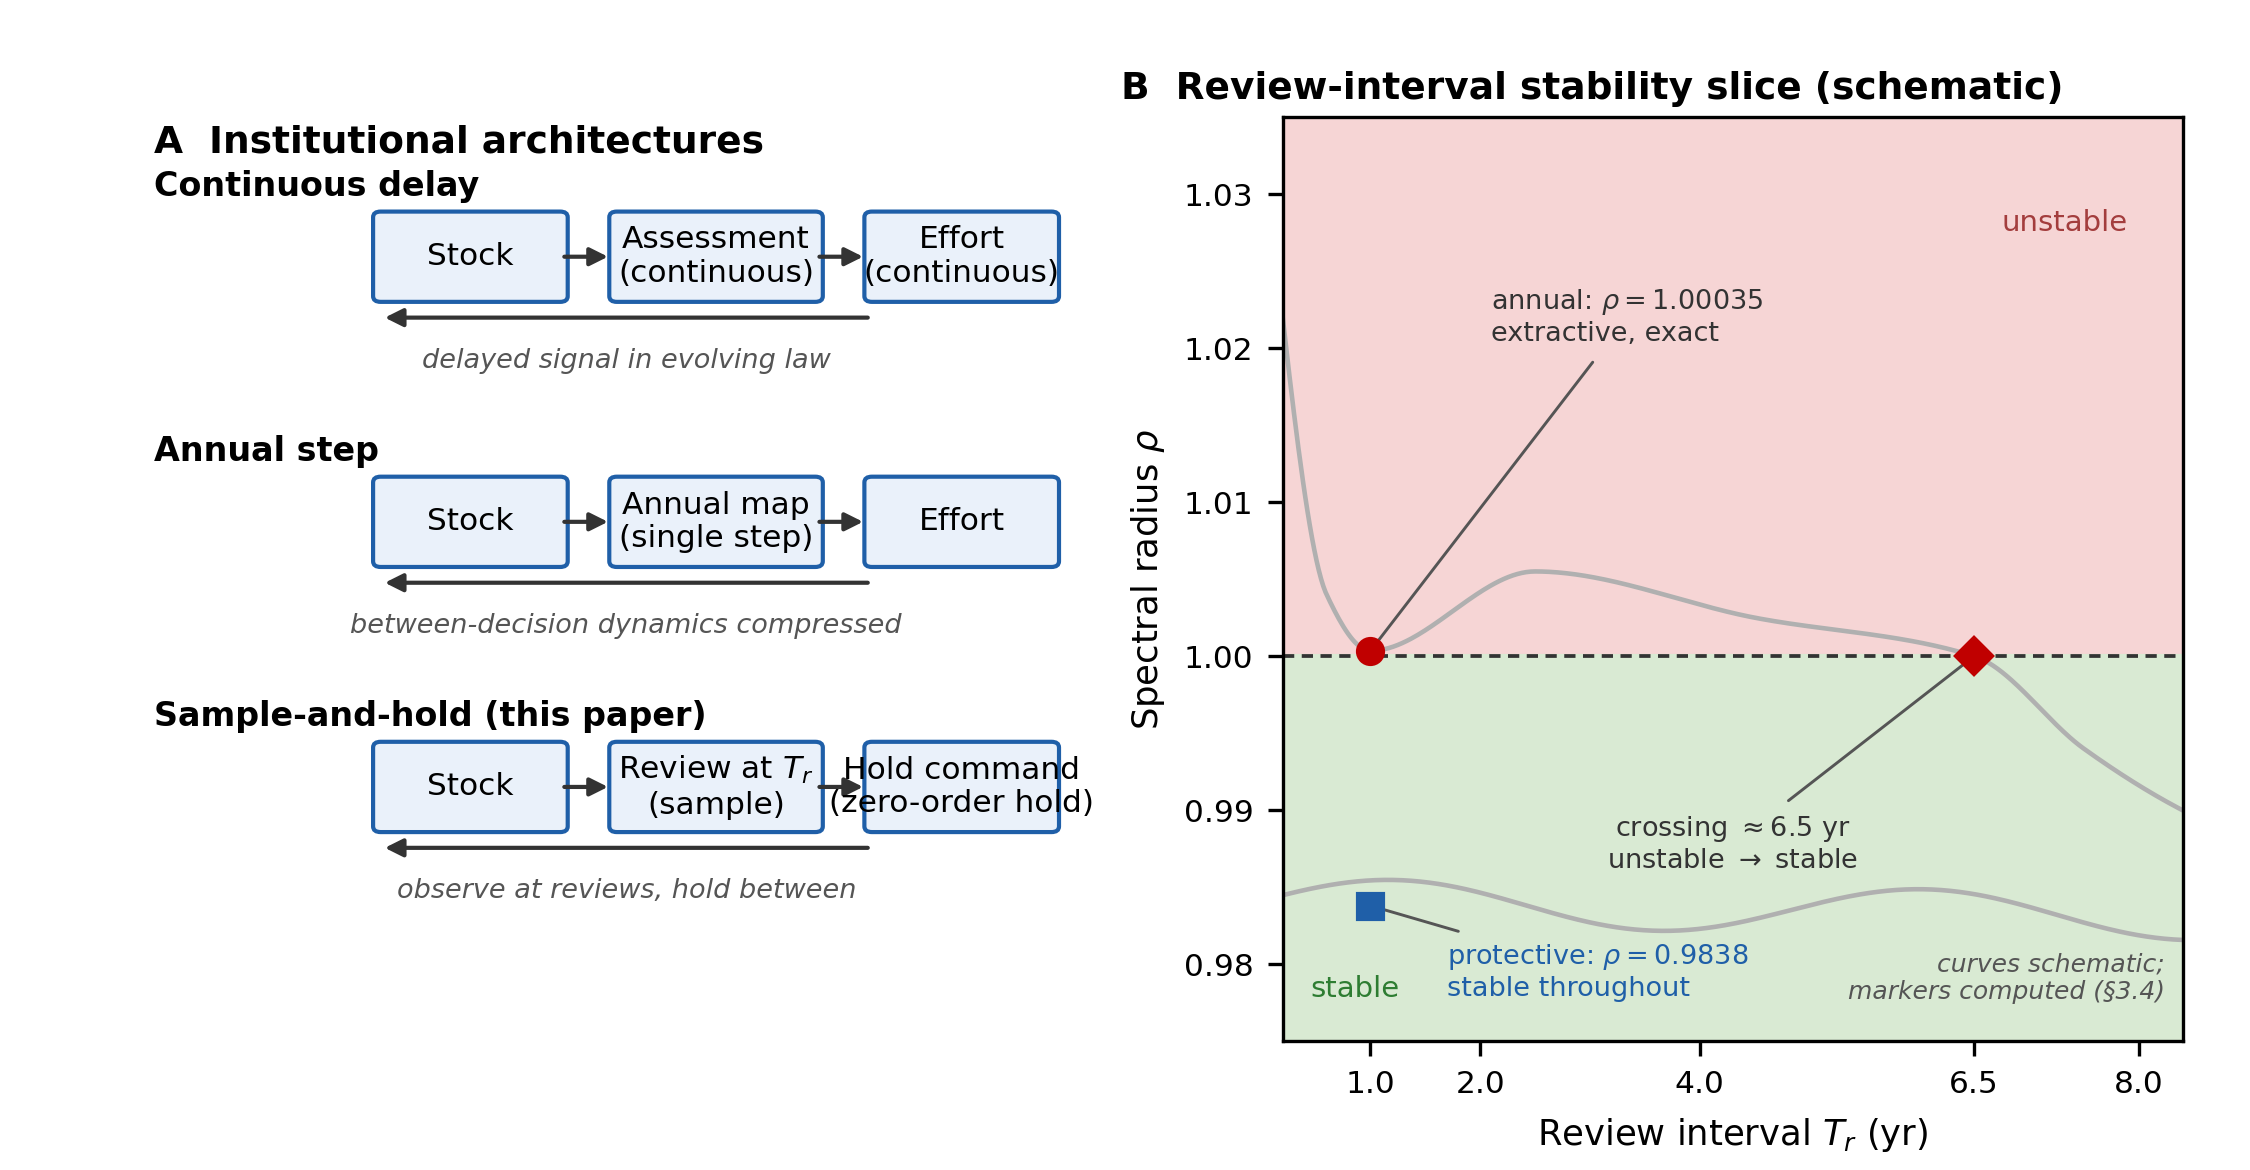
\includegraphics[width=\linewidth]{figs_p5/fig_concept_v38.png}
\caption{The decision clock. \textbf{A:} Three institutional architectures: continuous-delay feedback, the annual-step compression, and sample-and-hold governance, which observes at review times and holds the command between them. \textbf{B:} Review-interval stability slice (schematic): the extractive exact update is marginally unstable at annual review (\(\rho=1.00035\)) and crosses once near a 6.5-year interval (unstable \(\to\) stable), while the protective update is stable throughout (\(\rho=0.9838\) at annual review). Curves are schematic; markers show computed values (Section 3.4).}
\label{fig:decision-clock}
\end{figure}

\subsection{2 Material and methods}\label{material-and-methods}

\subsubsection{2.1 The sample-and-hold model of periodic
review}\label{the-sample-and-hold-model-of-periodic-review}

The model treats periodic review as a sample-and-hold control
architecture: the command set at a review instant is held fixed until
the next review, and only the between-review ecological dynamics are
continuous in time. Seven time objects are kept distinct, and no two are
collapsed into a single ``governance lag'' unless the empirical record
cannot resolve them and the aggregation rule is stated (Table 1).

For fisheries readers, the control-theoretic vocabulary maps onto management-procedure language: the controller is the harvest control rule; the command is the catch or effort limit it sets; the review interval is the advice cycle; the hold is the plan period between revisions; and the operator --- the decision architecture on which a stability claim is computed --- is the management procedure itself. Assessment error and implementation error enter where observation meets advice and where decisions meet deployment (Table 1).

\textbf{Table 1.} The governance-time ontology.

\begin{longtable}[]{@{}
  >{\raggedright\arraybackslash}p{(\columnwidth - 2\tabcolsep) * \real{0.5000}}
  >{\raggedright\arraybackslash}p{(\columnwidth - 2\tabcolsep) * \real{0.5000}}@{}}
\toprule\noalign{}
\begin{minipage}[b]{\linewidth}\raggedright
Object
\end{minipage} & \begin{minipage}[b]{\linewidth}\raggedright
Definition
\end{minipage} \\
\midrule\noalign{}
\endhead
\bottomrule\noalign{}
\endlastfoot
Observation interval \(T_{\rm obs}\) & Time between raw measurements \\
Assessment interval \(T_{\rm assess}\) & Time between formal state
estimates \\
Review interval \(T_r\) & Time between opportunities to change the
command \\
Decision lag \(\tau_{\rm dec}\) & Assessment completion to formal
decision \\
Deployment lag \(\tau_{\rm dep}\) & Decision to implemented change in
extraction pressure \\
Ecological response lag \(\tau_{\rm eco}\) & Implementation to
detectable ecological response \\
Memory timescale \(\tau_m\) & Relaxation time of a filtered
institutional signal; not a discrete delay \\
\end{longtable}

\[ \text{observation} \to \text{assessment} \to \text{advice} \to \text{decision} \to \text{implementation} \to \text{ecological response} \] The chain is the sequence Table 1 resolves into distinct objects; collapsing any two stages without a stated aggregation rule is the measurement-level form of architecture substitution.

Reviews can be annual while deployment
is delayed; observations can be frequent while decisions are legally
fixed for several years; and stock and realised-effort series alone may
identify only a combined closed-loop phase shift rather than the
separate \(\tau_{\rm dec}\) and \(\tau_{\rm dep}\). Separating them
empirically requires dated observation releases, assessment products,
commands, and implementation records. Alternatively, a proved
structural-identifiability argument for the specified observation model
can serve. Two further conventions apply. The review
opportunity is not the same as the response sign: the extractive command
studied here raises effort in response to a perceived decline, and the
protective controller enters only as a comparator. The fixed-\(\tau\)
form is also an idealisation. Real institutions confronting visible
scarcity typically change their instrument set --- buyouts, engineered
transfers, new infrastructure --- rather than hold a single response law
with constant delay. Any estimated \(\tau\) therefore summarises a
changing control architecture, not a structural constant.

\textbf{Box 1. Management regimes as sample-and-hold architectures.}

Four institutional regimes in the review--hold vocabulary.

\begin{longtable}[]{@{}
  >{\raggedright\arraybackslash}p{(\columnwidth - 10\tabcolsep) * \real{0.2000}}
  >{\raggedright\arraybackslash}p{(\columnwidth - 10\tabcolsep) * \real{0.2000}}
  >{\raggedright\arraybackslash}p{(\columnwidth - 10\tabcolsep) * \real{0.2000}}
  >{\raggedright\arraybackslash}p{(\columnwidth - 10\tabcolsep) * \real{0.2000}}
  >{\raggedright\arraybackslash}p{(\columnwidth - 10\tabcolsep) * \real{0.2000}}@{}}
\toprule\noalign{}
\begin{minipage}[b]{\linewidth}\raggedright
Regime
\end{minipage} & \begin{minipage}[b]{\linewidth}\raggedright
Review
\end{minipage} & \begin{minipage}[b]{\linewidth}\raggedright
Instrument
\end{minipage} & \begin{minipage}[b]{\linewidth}\raggedright
Hold
\end{minipage} & \begin{minipage}[b]{\linewidth}\raggedright
Emergency clause
\end{minipage} \\
\midrule\noalign{}
\endhead
\bottomrule\noalign{}
\endlastfoot
Annual TAC fishery & 1 yr & TAC (quota) & 1 yr & in-year adjustment where provided \\
Multiannual plan & 3--5 yr & fishing-mortality rule & multi-year & trigger review \\
Moratorium & indefinite & closure & until review & reopening rule (Section 3.8) \\
Data-limited system & irregular & effort controls & variable & crisis response \\
\end{longtable}

\emph{Notation.} Throughout, \(N\) denotes the resource stock, \(Z\) the
institutional deficit signal, and \(E\) the extraction effort. The
review Poincar\'e map --- the discrete-time map obtained by sampling the
continuous flow at review instants --- is written \(\mathcal P_{T_r}\);
its Jacobian at the fixed point \(X^*\), the monodromy matrix of the
sampled loop, is \(D\mathcal P_{T_r}(X^*)\) (Section 2.3's multiplier
condition is written on it); the projection onto the admissible effort
interval \([0,E_{\max}]\) is \(\Pi_{[0,E_{\max}]}\). The signal map
\(\Phi\) is a nonnegative functional of the deficit, with memory
timescale \(\tau_m>0\); its softplus realisation is \(\Phi_k\), with
shift \(\delta = \log 2/10 \approx 0.069\) and sharpness \(k\) (the shift is the equilibrium memory level, distinct from and unrelated to the effort-law
gain \(\delta_0\), as the display below states). The effort law is
\(F_B\). The assessment operator is \(\mathcal A_n\) and the observation
operator is \(\mathcal O\). In the control sections \(S(\cdot)\) is
surplus production --- \(S(N)\) on the logistic plant (defined after equation (2)) and
\(S(A)\) on the stage plant (Section 3.4) --- while \(g\) (Section 3.3),
\(C_E\) and \(C_Z\) (Section 3.4), and the four-state loop (Section 3.7)
are defined where they are used. In the northern cod case (Sections 2.7
and 3.8, Table 2) \(S\) is instead spawning stock biomass (reported as
SSB in Table 2), \(\mathfrak s\) the unstable threshold, \(K\) the
unexploited carrying capacity, \(C(t)\) removals, \(M\) instantaneous
natural mortality (with extra mortality \(M_x\) in Lemma 2.2), and \(F\)
fishing mortality. The two scopes of \(S\) never share an equation, and
no other symbol serves two sorts: the monodromy is written
\(D\mathcal P_{T_r}(X^*)\) throughout, and Lemma 2.2's production
maximum is written \(f_{\max}\), leaving \(M\) to natural mortality
alone. Symbols are tabulated with their definition sites in Table 4 of
Appendix A.

Let review times be \(t_n=nT_r\). Between reviews, extraction effort is
held at \(E_n\) and the resource stock follows the logistic process
under held effort:

\[
\dot N(t)=rN(t)\left(1-\frac{N(t)}{K}\right)-qE_nN(t),\qquad t\in[t_n,t_{n+1}),
\tag{1}
\]

while the institutional signal \(Z\) is the filtered nonnegative deficit

\[
\dot Z(t)=\frac{\Phi\bigl(qE_nN(t)-S(N(t))\bigr)-Z(t)}{\tau_m},\qquad \tau_m>0,
\tag{2}
\]

with \(S(N)=rN(1-N/K)\) the surplus production and \(\Phi\ge 0\) a
nonnegative signal map with memory timescale \(\tau_m\). The assessment
available at review \(n\) is

\[
\widehat Z_n=\mathcal A_n\!\left(\{Y_j:t_j\le t_n-\tau_{\rm dec}\}\right),\qquad
Y_j=\mathcal O\bigl(N(t_j)\bigr)+\varepsilon_j,
\tag{3}
\]

which separates the latent process \(N\), the observations \(Y\), and
the assessments \(\widehat Z\). Measurement and assessment errors need
not be independent or Gaussian, but the admissible error support is
restricted to \(\widehat Z_n \ge 0\). The multiplicative-error
robustness experiment of Section 3.3 satisfies this by construction. In the executed calibration all parameters entering the effort law are positive (\(r\), \(K\), \(q\), \(E_{\max}\), \(\Delta_{\rm ref}\), \(Z_{\rm ref}\), \(\tau_m > 0\)); because \(Z_{\rm ref} > 0\) and \(\widehat Z_n \ge 0\), the rational term is well defined on the admissible state space. The effort law's rational term is undefined at
\(\widehat Z_n = -Z_{\mathrm{ref}}\) and changes sign beyond it, and
projection of the final command does not repair an undefined update. In
the baseline deterministic record the assessment operator is exact and
contemporaneous, \(\widehat Z_n = Z(t_n^-)\): each command uses the just-flowed end-of-period state, indexed by the review that reads it (\(\widehat Z_{n+1}\) in (4)); the exact update holds this same flowed value. The review map is the
projected forward-Euler step

\[
E^{\rm cmd}_{n+1}=\Pi_{[0,E_{\max}]}\left\{E_n+T_rF_B(E_n,\widehat Z_{n+1})\right\},
\tag{4}
\]

--- one specific reviewed controller among many (direct command rules,
exact integration under held assessment, incremental rules with fixed
step). Because the increment scales with \(T_r\), a sweep in \(T_r\)
changes both the hold duration and the accumulated gain per review. The
separating computation is the exact held-assessment update (the exact update), reported in
Section 3.4 with attribution to the companion delay study (Abaee, 2026). The effort law is

\[
F_B(E,Z)=\left(1-\frac{E}{E_{\max}}\right)
\left[
\eta E\left(\frac{Z}{\Delta_{\rm ref}}-\frac{E}{E_{\max}}\right)
+\delta_0\frac{Z}{Z_{\rm ref}+Z}
\right],
\]

The protective comparator is the quota-tracking law

\[
F_B^{\rm prot}(E,Z)=\left(1-\frac{E}{E_{\max}}\right)
\eta_p\bigl(E_{\rm cap}(Z)-E\bigr),
\qquad
E_{\rm cap}(Z)=E_0\frac{Z_{\rm ref}}{Z_{\rm ref}+Z},
\]

with \(\eta_p = \eta\) and \(E_0 = E^*(Z_{\rm ref}+\delta)/Z_{\rm ref}\), calibrated so its unique interior rest coincides with the extractive fixed point; its linearised gains there are \(C_E = -0.850336\), \(C_Z = -1.661702\) (Abaee, 2026, equation~(3)), reviewed through the same projection \(\Pi_{[0,E_{\max}]}\). At \(E=0\) the law commands \(\eta_p E_{\rm cap}(Z)>0\), so zero effort is not absorbing; saturation at \(E_{\max}\) is through the gate and the projection.

together with the shifted, floored softplus signal map

\[
\Phi_k(s)=\max\left\{0,\ \frac{1}{k}\log\!\bigl(1+e^{ks}\bigr)-\frac{\log 2}{k}+\delta\right\}.
\]

with shift \(\delta = \log 2/10 \approx 0.069\), the equilibrium memory level (\(Z^* = \Phi(0) = \delta\); distinct from
and unrelated to the effort-law gain \(\delta_0\)) and sharpness \(k\)
--- the value used in the computed records, \(k = 10\), is stated where it is used in Section 3.4 and collected in Table 3 of Appendix A. The
multiplier records of Section 3.4 presuppose a fixed point interior to
the nonsmooth regions of \(\Phi_k\) and \(\Pi_{[0,E_{\max}]}\):
\(\Phi_k(0) = \delta\) gives the equilibrium deficit \(s^* = 0\)
uniquely, with softplus slope \(sp_k'(0) = 1/2\), and \(E^* = 2.09\)
lies in the interior \((0, E_{\max})\); the coordinates
\((89.55188, \delta, 2.08962)\) are listed in Table 3 of Appendix A.

Equations (1)--(4) with \(\Phi=\Phi_k\) constitute the extractive
controller studied throughout. It is an explicit controller
discretisation, not a generic harvest-control rule and not a model of
protective quota reduction. Three comparators are distinctly specified: the protective controller (the quota-tracking law above, the same machinery with the
response to decline entering with the opposite sign), the fixed-plan
controller (no state-responsive update between scheduled resets), and
the hybrid controller (annual-change limits, emergency triggers, or
legal overrides). The comparators are specified for the prospective
management-strategy evaluation (Section 4.5), not presented as completed
experiments. A fixed plan and a state-responsive plan with the same
nominal review period are not the same intervention. The model-level run
of the comparator evaluation on the logistic hold-map core --- the plant
of the closed-form operator results --- is executed and reported in
Section 3.4 at the stated evidential status (deterministic,
seed-fixed, on the specified architecture only). The prospective
real-system design of Section 4.5 remains unexecuted.

\subsubsection{2.2 Registration
conventions}\label{registration-conventions}

The deterministic record fixes a one-step flow-then-update convention,
stated in pre-review/post-review terms. On \([t_n, t_{n+1})\) effort is
held at \(E_n\). At the review instant \(t_{n+1}\) the contemporaneous,
exact assessment \(\widehat Z_{n+1} = Z(t_{n+1}^-)\) of the flowed state
is read (\(\tau_{\rm dec}=\tau_{\rm dep}=0\)), and equation (4) computes
the command \(E_{n+1}\) held on the following interval. The pre-review
state is \(X_n^-=(N(t_n^-),Z(t_n^-),E_{n-1})\) and the map used is
the pre-review Poincar\'e map \(X_{n+1}^-=\mathcal P_{T_r}(X_n^-)\). The
reversed ordering (command first, flow second) is a different hybrid
system and is not used. No decision or deployment queue is present, and
multiplicative assessment error enters only the designated robustness
experiment. A positive \(\tau_{\rm dep}\) requires an explicitly
specified hold or interpolation rule.

The computational status of the response-region records is stated with
the same care. Classification used long-horizon trajectories, tail
amplitudes, multiple histories, and integration-step refinement. It did
not use Poincar\'e-map multipliers, monodromy matrices, or Floquet
multipliers. The reported bands are therefore finite-grid,
trajectory-classified response regions, and no Neimark--Sacker, flip, or
other multiplier-crossing classification is claimed. Until the solver
configuration and initial histories are attached (Appendix A), the
stage-output values carry provisional status. For the logistic hold-map
core the multiplier-based boundary calculation is reported in Section 3.4. For the
stage-structured map the boundary record is supplied by the labelled
reconstruction of Section 3.4 --- a newly specified, pre-registered
object whose full specification (flow/update ordering, information
pattern, derivative construction, multiplier trajectories, nonlinear
trajectories, solver configuration) is given there. The original
stage record remains unattached, and its output values keep provisional
status. The computational requirements of this
section and of Sections 2.4, 2.5, 3.3, and 3.4 --- solver
configurations, initial histories, stock identifiers, the eligibility
table, the null-calibration record, simulation code and seeds, and the
reconstruction's plan, code, and output tables --- are consolidated in
Appendix A, which also fixes the pre-registration convention.

\subsubsection{2.3 The review-map
operators}\label{the-review-map-operators}

Three objects are in play: the continuous-delay equation, the logistic
hold map, and the stage-structured review map. The continuous delay
equation and the logistic sample-and-hold map are the same feedback loop
under two delay operators. The stage-structured map is a different
ecological plant (delayed-recruitment stage structure against scalar
logistic surplus production) with a different state dimension; it is not
an operator substitution on the logistic plant. A valid architecture
comparison holds the ecological plant, controller linearisation,
equilibrium, and parameter vector fixed while changing only the timing
operator. The 3--4 yr windows and the \(\approx 6.5\) yr exact-update crossing below
are therefore reported as a comparison across plants and operators, which does not isolate the operator effect; the one-plant operator contrast in Section 3.4 isolates the operator for the logistic plant. Changing the
operator can move or delete a crossing, and that relocation is a
property of the review map's spectrum, not a refutation of the loop mechanism. The
discipline throughout is that every stability statement names its
operator, and statements computed on the hold map, on the
stage-structured review map, and on the continuous-delay equation do not
transfer to one another. The operative condition is
\(\det(D\mathcal P_{T_r}(X^*)-e^{i\theta}I)=0\) on the map to which the
statement refers, with \(D\mathcal P_{T_r}(X^*)\) the Jacobian of the
review map at its fixed point (the monodromy matrix of the sampled
loop).

For a deterministic sampled system, the inter-review flow and the review
update combine into a Poincar\'e map \(X_{n+1}=\mathcal P_{T_r}(X_n)\),
where \(X_n\) includes the ecological state, memory, held command, and
any explicitly modelled queue. A fixed point is locally asymptotically
stable if and only if every eigenvalue of \(D\mathcal P_{T_r}(X^*)\)
lies inside the unit disk. A verified crossing through the unit circle
as the fixed parameter \(T_r\) changes is a sampled-data parameter
bifurcation. It is not rate-induced tipping, which requires a
nonautonomous parameter path and a loss of tracking as the ramp speed
changes (Ashwin, Wieczorek, Vitolo, and Cox, 2012).

\subsubsection{2.4 The cross-sectional spectral
screen}\label{the-cross-sectional-spectral-screen}

The screen's input layer is a fixed 42-stock cohort of the RAM Legacy
Stock Assessment Database v4.66 (Ricard, Minto, Jensen, and Baum, 2012): the annual-review designation (applied from general regime knowledge, not per-stock primary verification) covers the full 58-stock panel, and 42 stocks pass the \(n\ge 20\) valid-point filter (series lengths 20--77 yr). The release
records stock and assessment metadata and series such as biomass,
fishing mortality or exploitation rate, total allowable catch, catch
advice, and effort. It does not encode controller sign, the decision
rule, or dated decision and deployment queues. The annual-review
designation is therefore a criterion applied in this analysis, not a
database classification of a stock as extractive or protective.

For each eligible biomass (spawning-stock biomass) series, the analysis
removes a linear trend, computes a Lomb--Scargle periodogram (Lomb, 1976;
Scargle, 1982), normalises it to unit total power, and integrates power in
prespecified bands: target bands A (2.5--5 yr, anchovy class) and B (5--9 yr,
sprat class), bracketing the observable-specific dominant biomass peaks near 4 and
8 yr of the archived stage-map diagnostics (provisional records, Section 3.3), with contextual bands C (9--14 yr, cohort/recruitment) and D (14--30 yr, trend/regime). No multiplier-crossing verdict depends on the archived diagnostics. The tested
statistic is band-integrated power, compared with a per-series AR(1) red-noise
null (coefficient by lag-1 autocorrelation of the linearly detrended series; 200 replicates, seed 7, detrending inside each replicate; Lomb-Scargle on 1,500 frequencies from \(1/(2\cdot{\rm span})\) to 0.5 yr\(^{-1}\)). Empirical
\(p\)-values over the 84 target-band cells (42 stocks by bands A and B) are
adjusted by the Benjamini--Hochberg false-discovery-rate procedure (Benjamini
and Hochberg, 1995), which controls the false discovery rate, not the
familywise error rate. Dependence across stocks (shared climate forcing,
shared assessment methods) is acknowledged (Benjamini and Yekutieli,
2001). The reported zero count is the
BH-adjusted result. A peak is classified as robust only if it survives the
null comparison and the multiplicity adjustment. The cohort table, screen
routine, and multiplicity reconstruction (\texttt{ram\_target\_stocks.csv},
\texttt{ram\_crosssection.py}, \texttt{verify\_bh.py}) are deposited with
the article. The screen is a restricted result: its weight is limited to
the refutation stated in Section 4.2, and its null verdict survives the
eleven-variant sensitivity battery of Supplementary S9.1.

\subsubsection{2.5 Power analysis}\label{power-analysis}

Power experiments inject the model-generated effort signal into
white noise (multiplicative lognormal, fractional \(\sigma\)) and apply the same band-power statistic. Formally the reported power is \(P({\rm reject}\mid{\rm injected\ signal})\) at the 5\% level over the design grid (the conventional power-analysis framing of Cohen, 1988). Power is estimated
on 100--200 yr synthetic records across noise scales. The demonstration
routine and grid driver with the executed configuration and seeds
(\texttt{power\_demo.py}, \texttt{power\_driver\_v2.py}) are deposited
with the article. The executed grid configuration is Supplementary S13.1.

\subsubsection{2.6 The structured case
search}\label{the-structured-case-search}

The case search is a curated inventory, not a systematic review.
It considered more than thirty systems spanning fisheries, aquaculture,
groundwater, surface water, rangeland, wildlife harvest, forestry, and
produced-capital markets, under four criteria:

\begin{enumerate}
\def\labelenumi{(\roman{enumi})}
\tightlist
\item
  a responsive institutional feedback rather than a one-time cap or ban;
\item
  an independently dateable response or implementation lag;
\item
  no major environmental, biological, or structural driver empirically
  supported as generating the same outcome, where the comparative rule
  is that a candidate institutional mechanism must outperform
  pre-registered alternatives on held-out prediction, phase ordering, or
  intervention response (since ``capable of generating'' is not a
  falsifiable exclusion in open ecological systems);
\item
  individual-resource or individual-station data rather than an
  aggregate series.
\end{enumerate}

Behind criterion (iii) is an explicit list of the alternative
mechanisms that can mimic or replace an institutional cycle:
stage/maturation delays and cohort resonance; recruitment suppression
versus stock culling; support-pool/nutrient limitation; pollution/waste
feedback; predator--prey or climatic forcing; and direct abiotic mining
and slow-store exhaustion. The rule is that a candidate institutional
mechanism must be compared with these alternatives rather than
identified from periodicity alone. No system in the searched set meets all four criteria; the case-screening table (32 systems) and query log are recorded in Supplementary S4.

\subsubsection{2.7 The northern cod case: constitutive model and
evidence}\label{the-northern-cod-case-constitutive-model-and-evidence}

The northern cod case (NAFO 2J3KL) is treated as a bounded empirical
object. Its illustrative constitutive model is the strong-Allee surplus
equation:

\[
\frac{dS}{dt}=rS\left(1-\frac{S}{K}\right)\frac{S-\mathfrak s}{K-\mathfrak s}-C(t),
\tag{5}
\]

with \(S\) the spawning stock biomass, \(r\) the intrinsic growth rate,
\(K\) the unexploited carrying capacity, \(\mathfrak s\) the unstable
threshold, and \(C(t)\) the removals. The Schaefer model is the
formal limit of this family (\(\mathfrak s\to-\infty\)) in which the factor
\((S-\mathfrak s)/(K-\mathfrak s)\) is replaced by \(1\). No value of
\(\mathfrak s\) makes the displayed factor identically \(1\) (it tends
to \(1\) only in the limit \(\mathfrak s\to-\infty\)), so the Schaefer
comparison is a change of growth law, not a parameter specialisation.
The constitutive equation is illustrative, not a fit --- and the obstruction class is the
one-dimensional autonomous equation with fixed parameters and fixed
removals. The displayed equation is autonomous exactly when removals are
fixed.

\textbf{Remark 2.1} (Phase-line obstruction). Let
\(f:\mathbb{R}\to\mathbb{R}\) be locally Lipschitz, and let \(x(\cdot)\)
be a nonconstant solution of the scalar autonomous ODE \(\dot x=f(x)\).
Then \(x\) is strictly monotone; it never attains an equilibrium value
and cannot cross an equilibrium in either direction. Consequently, an
exact path that repeatedly rises and falls across a common interval is
incompatible with any single fixed scalar autonomous model.

\emph{Proof.} If \(x\) is nonconstant on an interval and
\(x(t_1)=x(t_2)\) with \(t_1<t_2\), then by Rolle's theorem there exists
\(\tau\in(t_1,t_2)\) with \(\dot x(\tau)=0\), i.e.~\(f(x(\tau))=0\). By
uniqueness the solution through \((\tau,x(\tau))\) is the constant
equilibrium solution, a contradiction. Hence every solution is strictly
monotone or constant. If a trajectory met an equilibrium value \(x^*\)
at any time, it would be constant thereafter and, by uniqueness applied
backwards, before; a nonconstant solution therefore never attains an
equilibrium value and cannot cross one in either direction. A path that
rises and falls across a common interval attains some level twice with
opposite directions, contradicting monotonicity. \ensuremath{\square}

\textbf{Lemma 2.2} (Extra-loss threshold shift, conditional).

\emph{Statement.} Assume \(0 < \mathfrak s < K\). (i) Constant loss. In the constitutive model with an
additional constant removal \(C>0\), the production function is replaced
by \(f_C(S)=f(S)-C\); the positive equilibria of the modified function
are the solutions of \(f(S)=C\), the smaller one (the effective
threshold) lies to the right of \(\mathfrak s\), and at the production
maximum the two positive equilibria coalesce and beyond it disappear ---
all conditional on the solutions existing, i.e.~on \(C\) being below the
production maximum. For \(C=0\) the smaller positive equilibrium is \(\mathfrak s\); the strict rightward shift holds for \(C>0\).

\begin{enumerate}
\def\labelenumi{(\roman{enumi})}
\setcounter{enumi}{1}
\tightlist
\item
  Proportional mortality. With extra mortality \(M_x>0\) the modified
  production is \(f_M(S)=f(S)-M_xS\); positive equilibria solve
  \(f(S)/S=M_x\), \(S=0\) remains an equilibrium (unlike case (i), where
  \(\dot S|_0=-C<0\) drives the model below zero unless the removal is
  constrained near zero or the state equation is modified), and the smaller modified positive root lies strictly above \(\mathfrak s\) (in \((\mathfrak s, S_h)\), where \(S_h\) is the vertex of the per-capita curve \(h(S) = f(S)/S\)).
\end{enumerate}

\emph{Proof.} The constitutive production
\(f(S) = rS(1-S/K)(S-\mathfrak s)/(K-\mathfrak s)\) vanishes exactly at
\(0\), \(\mathfrak s\), \(K\); it is negative on
\((0,\mathfrak s)\cup(K,\infty)\), positive on \((\mathfrak s,K)\), and
its derivative vanishes exactly at
\[S_{\pm} = \frac{K+\mathfrak s \pm \sqrt{K^2-\mathfrak s K+\mathfrak s^2}}{3}, \qquad 0 < S_- < \mathfrak s < S_+ < K,\]
so \(f\) has exactly one critical point in \((\mathfrak s,K)\) --- the
unique maximum \(S^* = S_+\) with value \(f_{\max} = f(S^*) > 0\) ---
and \(f\) is strictly increasing on \((\mathfrak s,S^*)\) and strictly
decreasing on \((S^*,K)\).

\begin{enumerate}
\def\labelenumi{(\roman{enumi})}
\item
  The equilibria of \(f_C(S) = f(S) - C\) solve \(f(S) = C\), so none
  lie outside \((\mathfrak s,K)\), where \(f \le 0 < C\). For
  \(0 < C < f_{\max}\), the intermediate value theorem on
  \([\mathfrak s, S^*]\)
  (\(f(\mathfrak s) = 0 < C < f_{\max} = f(S^*)\)) and on \([S^*, K]\)
  (\(f(K) = 0 < C < f_{\max}\)) supplies one root in each interval, and
  strict monotonicity makes each root unique. The smaller root satisfies
  \(S_1(C) \in (\mathfrak s, S^*)\) --- the effective threshold lies
  strictly to the right of \(\mathfrak s\). As \(C \uparrow f_{\max}\)
  the two roots approach \(S^*\) from either side (coalescence), and for
  \(C > f_{\max}\) the equation \(f(S) = C\) has no solution: the two
  positive equilibria have disappeared.
\item
  Write \(f_M(S) = f(S) - M_x S = S\, (h(S) - M_x)\) with
  \(h(S) = f(S)/S = \frac{r}{K-\mathfrak s}(1-S/K)(S-\mathfrak s)\), a
  quadratic with roots \(\mathfrak s\) and \(K\), negative on
  \((0,\mathfrak s)\cup(K,\infty)\), and unique maximum \(H = h(S_h)\)
  at the vertex \(S_h = (\mathfrak s+K)/2\). Then \(f_M(0) = 0\): zero
  remains an equilibrium in every case. The positive equilibria solve
  \(h(S) = M_x\); for \(0 < M_x < H\) the same two-interval argument
  gives exactly two roots, the smaller in \((\mathfrak s, S_h)\) --- the
  threshold shift --- with coalescence at \(M_x = H\) and disappearance
  for \(M_x > H\), where \(f_M(S) = S(h(S)-M_x) < 0\) on \((0,\infty)\).
\end{enumerate}

In case (i), by contrast, \(f_C(0) = -C < 0\), so \(\dot S|_0 = -C\)
drives the state below zero unless the removal is constrained near zero
or the state equation is modified --- as claimed. \ensuremath{\square}

The case evidence is the assessment record (the recovery-potential and
sequential stock assessments: DFO, 2011, 2016, 2022, 2024). The crash
window (1991--1995) and the subsequent windows are documented by the
assessment table of DFO CSAS SAR 2016/026 (Table A2), produced by the
Northern Cod Assessment Model (NCAM; Cadigan, 2016), together with the
dated governance events (the moratorium announcement of 2 July 1992; the
reopening of 26 June 2024 with a total allowable catch of 18 kt). The
survival column \(\exp(-M)\) is a transformation of the reported
instantaneous mortality estimate, not an independently observed survival
series.

\subsection{3 Results}\label{results}

\subsubsection{3.1 Forward invariance of the sampled
process}\label{forward-invariance-of-the-sampled-process}

A first well-posedness check on the sampled controller is that the state
space on which the sample-and-hold dynamics act --- nonnegative stock,
nonnegative memory signal, admissible effort --- is preserved by the
review map. This check comes first because every
later result relies on the state remaining inside this set between
reviews.

\textbf{Proposition 3.1} (Forward invariance of the sampled process).
Assume:

(H0) \(r,K,q,E_{\max},\tau_m,Z_{\rm ref},\Delta_{\rm ref}>0\).

(H1) \(N(0)\ge 0\), \(Z(0)\ge 0\), \(E_0\in[0,E_{\max}]\).

(H2) The signal map \(\Phi\) is non-negative.

(H3) Every effort command is projected by \(\Pi_{[0,E_{\max}]}\).

(H4) Any between-review deployment interpolation remains in the convex
interval joining consecutive commands. The main model takes \(E(t)=E_n\), which satisfies (H4) trivially; the proposition is stated for the hold-or-interpolate class.

Then \(N(t)\ge 0\), \(Z(t)\ge 0\), and \(E(t)\in[0,E_{\max}]\) for every
time at which the sampled solution exists.

\emph{Proof.} Proceed by induction over review intervals. Suppose that
at a review time \(t_n\) one has \(N(t_n)\ge 0\), \(Z(t_n)\ge 0\), and
that the command to be held or interpolated lies in \([0,E_{\max}]\).
Projection places the next command in the same closed interval; a hold
retains an endpoint of that interval, and any convex interpolation
\(E(t)=(1-\theta(t))E_n+\theta(t)E_{n+1}\) with \(0\le\theta(t)\le 1\)
also remains in \([0,E_{\max}]\). On \([t_n,t_{n+1}]\), Eq. (1) gives

\[
N(t)=N(t_n)\exp\left\{\int_{t_n}^{t}\left[r\left(1-\frac{N(s)}{K}\right)-qE(s)\right]ds\right\}>0
\]

for a positive initial value, while if \(N(t_n)=0\), uniqueness gives
the identically zero solution on the interval; \(N\) cannot become
negative. Set \(\nu(t)=\Phi(qE(t)N(t)-S(N(t)))\ge 0\). Variation of
constants in Eq. (2) with \(\tau_m>0\) gives

\[
Z(t)=e^{-(t-t_n)/\tau_m}Z(t_n)+\frac{1}{\tau_m}\int_{t_n}^{t}e^{-(t-s)/\tau_m}\nu(s)\,ds\ \ge 0 .
\]

Boundedness from above holds automatically on the stock equation and is used
in the induction: on \([t_n, t_{n+1})\) the stock solves the
logistic equation under held effort, and \(\dot N \le 0\) at \(N = K\)
(the harvest term is non-negative), so \(N(t) \le \max\{N(t_n), K\}\)
throughout the interval. All three inequalities therefore hold through
\(t_{n+1}\); they hold at \(t_0=0\) by hypothesis, and induction proves
them on every review interval for which the sampled solution exists. \ensuremath{\square}

Positivity, boundedness, persistence above a threshold, and viability
are distinct properties; Proposition 3.1 establishes positivity and
effort admissibility only. The institutional implication is modest but
essential: the projected Euler step does not push the state outside
its specified admissible set on a single review interval, and any later
stability or instability claim is therefore a statement about dynamics
inside that set, not about escape from it.

\subsubsection{3.2 The rapid-review limit and what it does not
establish}\label{the-rapid-review-limit-and-what-it-does-not-establish}

Define \(u=(N,Z,E)\) and the continuous no-delay system \(\dot u=G(u)\)
assembled from Eqs. (1)--(2) with the effort law evaluated continuously.
Suppose \(G\) is continuously differentiable with bounded derivative on
a compact neighbourhood containing the compared trajectories on
\([0,T]\), assessments equal the contemporaneous state, no additional
decision or deployment queue is present, projection is inactive, and the
sampled and continuous systems share the initial state. The
frozen-effort flow followed by the explicit effort step then has a
one-step defect of order \(O(T_r^2)\) relative to the exact flow of
\(G\). The usual discrete Gronwall estimate yields an \(O(T_r)\)
review-time error and uniform convergence on every fixed finite horizon
as \(T_r\to 0\) (the sampled-data approximation framework of Ne\v{s}i\'c and
Teel, 2004).

This is a numerical-approximation property, not a finite-review
stability theorem. It gives no uniform-in-time estimate, does not
preserve stability automatically, and does not control any
trajectory-classified response region reported below. It excludes active
projection, delayed or erroneous assessment, a deployment queue, and
stochastic updates. In particular, it neither identifies a finite
\(T_r\) with a continuous discrete delay nor implies that sufficiently
small positive \(T_r\) is stable when the continuous target is unstable.
The converse caution is equally important. Under the additional
assumptions of hyperbolicity of the continuous equilibrium and
\(C^1\)-consistency of the sampled map with projection inactive locally,
the multipliers satisfy \(\mu_j(T_r) = 1 + T_r\lambda_j(A) + O(T_r^2)\)
(Stuart and Humphries, 1996), so local stability persists for all sufficiently small positive review intervals provided every continuous eigenvalue satisfies \(\Re\lambda_j<0\); if any \(\Re\lambda_j>0\), the sampled equilibrium inherits instability for sufficiently small \(T_r\). The finite-horizon result therefore neither proves nor
refutes stability transfer; the transfer hypotheses are what any such
claim would have to supply. The institutional reading is that ``rapid
review'' is not a stability guarantee --- a governance loop that reviews
frequently approximates a continuous controller only on finite horizons,
and the question of whether short review intervals stabilise or
destabilise the equilibrium is decided by the spectrum of the map, not
by the rapid-review limit.

\subsubsection{3.3 Response regions of the delayed-recruitment review
maps}\label{response-regions-of-the-delayed-recruitment-review-maps}

The delayed-recruitment records, classified from long-horizon
trajectories on the stage-structured review map, locate exploratory
response regions by stock class (the delayed-recruitment oscillation
literature of Gurney, Blythe, and Nisbet, 1980, supplies the classical
reference point). These are archived records whose generating
computation was never attached (Section 2.2): they are reported below at
provisional status, and the
pre-registered stage-map reconstruction of Section 3.4 does \textbf{not}
reproduce the multi-year windows on the anchovy- or sprat-class
parameterisation of that plant (reporting convergence there, with a
separate long-horizon band that has no archived counterpart). The
regions below are therefore archived, unreproduced records, not results
of the reconstructed object:

\begin{itemize}
\tightlist
\item
  \textbf{Anchovy-class:} persistent tail oscillation near
  \(T_r\approx 3\)--\(4\) yr, with a weak response at \(T_r=2\) yr;
  annual-review trajectories converge over the tested grids for every
  tested effort-response value.
\item
  \textbf{Sprat-class:} persistent tail oscillation near
  \(T_r\approx 6\)--\(12\) yr.
\item
  \textbf{Cod-class:} trajectories converge to equilibrium for every
  tested \(T_r\in[1,20]\) yr, although the corresponding
  continuous-delay calculation has an oscillatory interval --- a
  convergence-over-tested-grid record, not a stability theorem for every
  history.
\item
  \textbf{Slow-stock class:} for \(r\in(0.01,0.05)\) yr\(^{-1}\),
  oscillation over part of the tested grid below approximately 20--30 yr
  and convergence at longer review intervals, with transition brackets
  between approximately 30 and 50 yr depending on \(r\). This one-sided
  pattern does not contradict rapid-review consistency: the continuous
  no-delay target is itself unstable over part of the slow-\(r\) regime,
  so small-\(T_r\) trajectories may approximate an unstable target on
  finite horizons. The record is conditional on the delayed-recruitment
  variant and is not a general claim that slower review stabilises
  governance; the dominant timescales are centuries (the archived slow-stock cohort cycle: \(P \approx 250{-}360\) yr), beyond the length
  needed to resolve multiple cycles in most institutional records.
\end{itemize}

The corresponding continuous-delay calculations on the
delayed-recruitment parameterisation --- \(g\) is its maturation delay,
and the response regions are located through the product \(rg\) ---
locate response regions near \(rg\approx 1.5\)--\(1.6\): for \(g=2\) yr,
\(r\in(0.77,0.81)\) yr\(^{-1}\) at \(\eta=0.914\) (the uncalibrated Candidate-A baseline; Appendix A) with a delay interval
of approximately 2.6--7.8 yr; for \(g=1\) yr, the high-\(r\) interval is
approximately 1.565--1.585 yr\(^{-1}\) with a delay interval of 1.6--3.5
yr. These are finite-grid trajectory summaries, not closed analytical
stability regions.

A \(\tau_0\) decomposition separates, within the delayed-recruitment
operator, cohort-driven from institutional-delay-induced crossings: at
\(g = 5\) yr and \(\eta = 0.914\) the raw \(r\)-window [0.0076, 0.3705]
narrows to the institutional-only [0.2660, 0.3285], and fish-range
crossings from 12 to 8, under \(\tau_0\)-stable classification by
nonlinear ground truth. The separation is within one operator; it does
not isolate the cross-operator effect compared in Section 4.1. The
\(g = 5\) middle band overlaps slow cod-class growth rates but remains
confounded with cohort resonance. That operator differs from Section
3.7's four-state loop. Full windows, the twelve-cell decomposition grid,
and the middle-band table are tabulated in Supplementary S9.2.

Multiplicative assessment-error experiments preserve the anchovy-class
trajectory region through 30\% error and produce no noise-induced
persistent tail oscillation at annual review in the tested ensemble.
This is a robustness summary for the specified multiplicative
perturbation only. The archived diagnostics carry observable-specific
dominant peaks --- approximately 4 yr in anchovy-class biomass with 12
yr in effort, and approximately 8 yr in sprat-class biomass with 60 yr
in effort. These are reported only as observable-specific dominant peaks
over the analysed windows: components of one stationary periodic orbit
cannot have different fundamental periods, and harmonics, subharmonics,
modulation, or transient spectral content are unresolved; no
decomposition has established whether the baseline term, signal
regularisation, or another controller component dominates these
responses. The archived amplitudes indicate percent-scale biomass
excursions and order-one effort excursions relative to equilibrium. The
exact percentages are not used as effect-size estimates, because the
archived record does not distinguish peak-to-peak range from
half-range and the approach to the large effort response contains a long
transient.

\subsubsection{3.4 The operator spectra}\label{the-operator-spectra}

The logistic hold-map core permits a closed-form expression for the held logistic flow; the linearised review map is then constructed from this flow, the signal dynamics, and the update derivatives. With effort held at \(E\), the logistic flow over one
review interval is, for \(a(E) = r - qE \ne 0\),
\[N(t_{n+1}^-) = \frac{a(E)\,N(t_n^-)\,e^{a(E)T_r}}{a(E) + \tfrac{r}{K}N(t_n^-)\bigl(e^{a(E)T_r} - 1\bigr)},\]
and \(N(t_n^-)\big/\!\bigl(1 + \tfrac{r}{K}N(t_n^-)T_r\bigr)\) for
\(a(E) = 0\). In computations, the limit branch is used when \(|a(E)| < 10^{-12}\). The signal flow enters through equation (2) with this
forcing, and the linearised pre-review monodromy is assembled from the
held-flow state transition, the assessment derivative at
\(Z(t_{n+1}^-)\), and the update derivative of equation (4). The exact
held-assessment controller --- the separating comparator that isolates
the Euler step --- is the exponential update (the exact update; its review map the exact map) \(e_{n+1} = e^{C_E T_r}e_n + \tfrac{e^{C_E T_r}-1}{C_E}C_Z z_n\) for
\(C_E \ne 0\), and \(e_{n+1} = e_n + T_r C_Z z_n\) for \(C_E = 0\), with
\(e_n = E_n - E^*\) and \(z_n = Z_n - Z^*\) the deviations from the compared fixed point --- the exact solution, over one review interval, of the
linearised effort law \(\dot e = C_E e + C_Z z\) with the flowed end-of-period assessment
\(z\) held, where \(C_E\) and \(C_Z\) are the coefficients of that
linearisation (the partial derivatives of \(F_B\) with respect to \(E\)
and \(Z\) at the compared fixed point; unrelated to the removals \(C\)
of the cod case), and equation (4)'s increment is the forward-Euler
discretisation of the same linear object. This comparator is analytical, not a proposed institutional rule. Comparing its monodromy with
the forward-Euler map's separates review cadence, zero-order holding,
and Euler discretisation. That comparison is reported here: executed and
verified on the companion delay study's identical hold map (Abaee, 2026; same effort-law bracket, same softplus signal, same
forward-Euler monodromy reproducing the 47.536 yr crossing reported
here), the exact-update annual spectral radius is \(\rho = 1.00035\)
(Euler 1.00055); the 47.536 yr and 79.143 yr crossings are command-step artefacts of the forward-Euler update;
the exact map's single unit-circle crossing is
\(\approx 6.5\) yr; and the restabilising direction is preserved.

On the logistic hold-map core, the undelayed equilibrium is already
unstable, so annual review is unstable. On the computed crossing set,
the sampled equilibrium has a complex unit-circle crossing --- the
spectral signature of a Neimark--Sacker bifurcation, nonlinear
nondegeneracy not verified --- at \(T_r^{\rm UC}=47.536\) yr under the
forward-Euler command step and at \(\approx 6.5\) yr under the exact update, with the same restabilising direction. For an institution implementing the incremental Euler rule these crossings are dynamically real; they are artefacts only relative to the exact update.

\textbf{The complete crossing record.} On the logistic
hold-map core the unit-circle crossing record over \([0.2, 200]\) yr is
complete (Figure 2). It is computed from the linearised pre-review
monodromy on a 200,001-point scan with bisection refinement (deterministic;
it reproduces the numbers reported here on the range they cover). The
forward-Euler update crosses twice on the extractive channel --- a
complex pair at \(T_r = 47.536\) yr (unstable \(\to\) stable) and a real
\(-1\) multiplier at 79.143 yr (stable \(\to\) unstable), stable band
\([47.536, 79.143]\) yr --- and once on the protective channel --- a real
\(-1\) at 2.306 yr (stable \(\to\) unstable), stable only on
\([0.2, 2.306]\) yr. The exact update crosses once on the
extractive channel --- a complex pair at 6.501 yr (unstable \(\to\) stable) at the baseline parameter vector (Table 3), stable on \([6.501, 200]\) yr --- and never on the protective
channel, which is stable at every tested interval with maximum spectral
radius 0.9967. Both Euler crossings of the extractive channel are
therefore command-step artefacts relative to the exact map's single
crossing, and the Euler protective instability beyond 2.306 yr is
likewise an artefact: the exact protective map is stable throughout.

\textbf{Spectral margins of the annual-review verdict.} The
annual-review instability is a near-unit-circle record, and its margins
are part of the record. The exact update's annual
spectral radius is \(\rho = 1.00035\) --- a modulus exceeding unity by
\(3.5\times 10^{-4}\) --- with the forward-Euler update at \(1.00055\)
and the protective channel at \(0.9838\) (maximum \(0.9967\) over the
tested range). The multiplier types are reported with the crossings ---
a complex pair at the exact map's single 6.501 yr crossing (the
Neimark--Sacker signature) and at the Euler extractive crossing (47.536 yr), and real \(-1\) multipliers at the Euler
crossings (79.143 yr extractive, 2.306 yr protective) --- while the
dominant multiplier's angle \(\theta\) at the crossing and the
continuous eigenvalue \(\lambda\) to which Section 3.2's transfer
relation refers are listed in Table 3 (Appendix A). At a margin of this size the
verdict is conditional on the monodromy's numerical construction --- the
stated precision record is the 200,001-point scan with bisection
refinement; the linearisation construction and floating-point detail are
archive items --- and on the parameter vector listed in Table 3. What
the margin does not affect is the ordering across updates and
channels (exact \(1.00035\) below Euler \(1.00055\); protective
\(0.9838\) below both) or the crossing directions; the annual-instability verdict is read at that status. Near-unit-circle behaviour of this size is read as high sensitivity of the verdict to the parameter vector, not as a robust claim about annual-review institutions in general.

\begin{figure}[htbp]
\centering
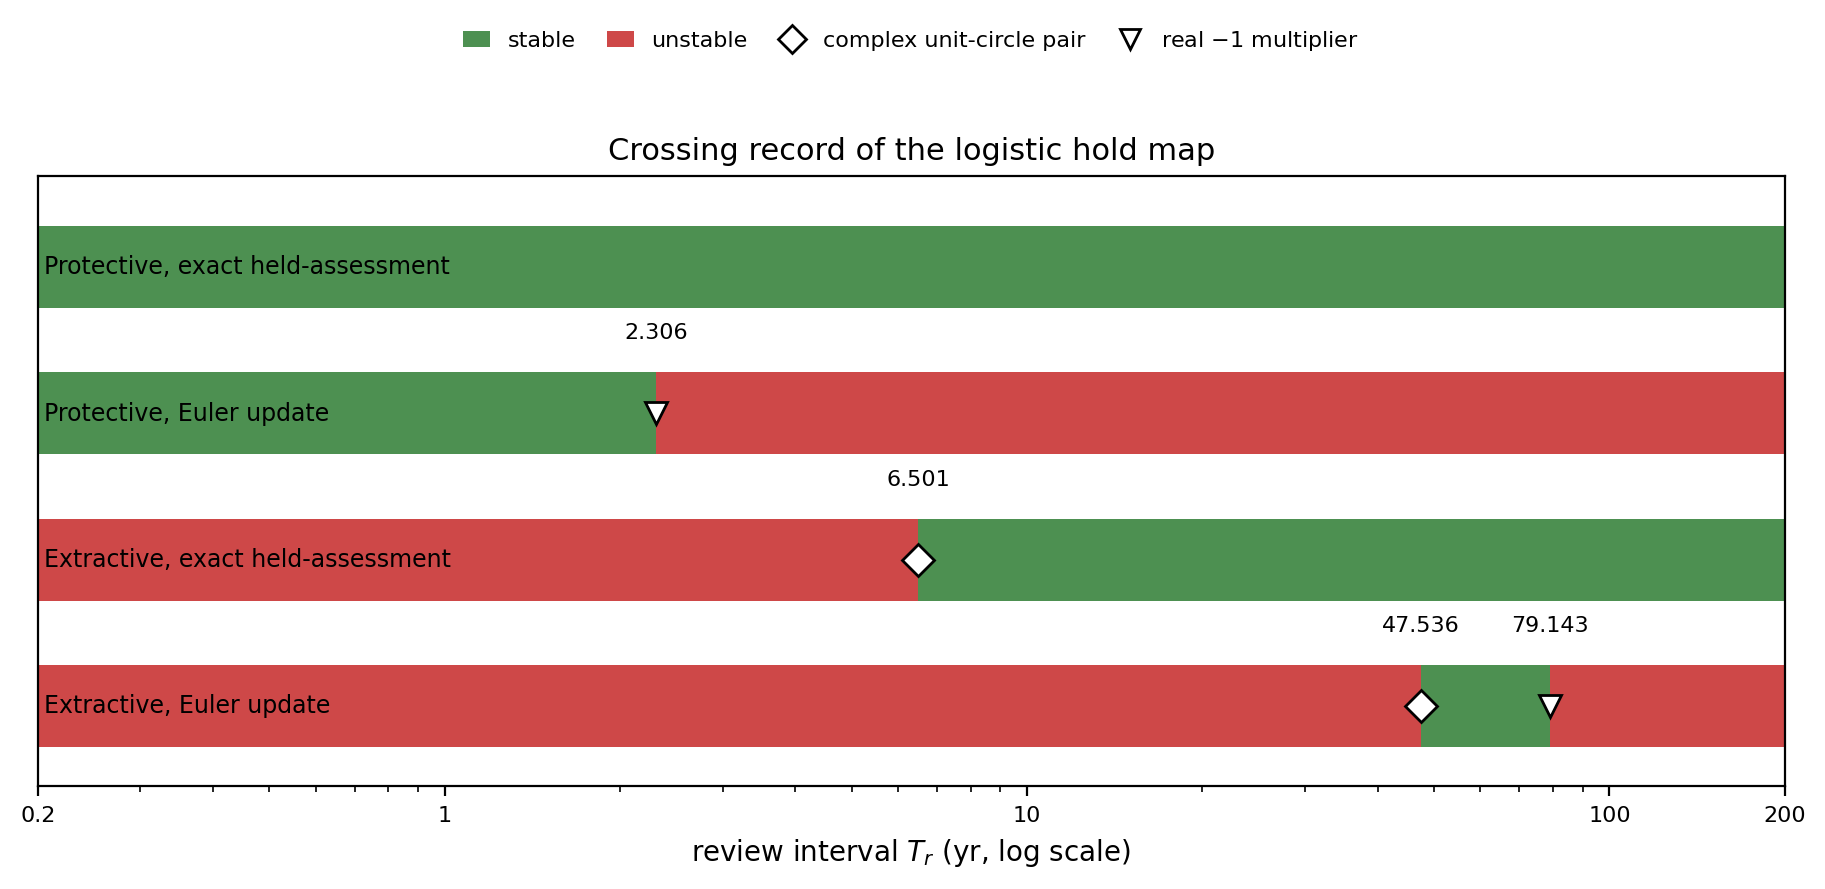
\includegraphics[width=\linewidth]{figs_p5/fig1_crossing_record_v25.png}
\caption{Crossing record of the logistic hold map: stable (green) and unstable (red) review-interval ranges for the four update \ensuremath{\times} channel combinations (forward-Euler and exact updates on the extractive and protective channels), with crossing markers (diamond: complex unit-circle pair; triangle: real \ensuremath{-}1 multiplier). Annual review is nominally unstable on both extractive updates (\(\rho=1.00035\) exact, \(1.00055\) Euler; protective \(0.9838\)), conditional on the numerical construction and parameter vector (Spectral margins paragraph); the Euler-reported 47.536 and 79.143 yr crossings are command-step artefacts relative to the exact update's single 6.501 yr crossing, and the protective Euler crossing at 2.306 yr is likewise an artefact --- the exact protective map is stable at every tested interval (maximum spectral radius 0.9967).}
\end{figure}

\textbf{The one-plant operator contrast.} With the crossing record
complete, the operator comparison can be made on one plant rather than
across plants. The same extractive loop under continuous delay carries
the companion delay study's certified Hopf pair at 3.666 and 150.358 yr
(Abaee, 2026); the sampled operator's exact crossing sits
at 6.501 yr. The companion's window is delay-stabilising, not
delay-destabilising: the undelayed loop is already unstable, the lower
crossing at \(\tau_- = 3.666\) yr is stabilising, the upper crossing at
\(\tau_+ = 150.358\) yr destabilising, and the loop is linearly unstable
for \(0 < \tau < \tau_-\) (Abaee, 2026). Annual review is
nominally unstable under sampling (\(\rho = 1.00035\), conditional on the numerical construction and parameter vector as stated above), and the same loop under
continuous delay is likewise unstable at \(\tau = 1\) yr; at \(T_r = 8\)
yr both operators are stable (the sampled loop restabilised above its
6.501-yr crossing, the continuous loop inside its stabilised window). The
operator contrast on one plant is an edge contrast: the sampled
operator's restabilising crossing (6.501 yr) sits above the continuous
operator's stabilising entry (3.666 yr), and the sampled loop's
stability persists to the 200-yr scan ceiling where the continuous loop
has already destabilised at \(\tau_+\) --- the operator moves both edges
of the stability window on the same plant, and the cross-plant
observation of Section 2.3 is a same-plant one.

\textbf{The undelayed limit, reconciled explicitly.} Three statements of
this manuscript bear on the undelayed loop and are read together.
Section 2.3 states the continuous-delay
equation and the logistic hold map to be the same feedback loop under
two delay operators; Section 3.2 states that under hyperbolicity the
sampled multipliers satisfy
\(\mu_j(T_r) = 1 + T_r\lambda_j + O(T_r^2)\), so that small-\(T_r\)
sampled stability follows the sign of \(\mathrm{Re}\,\lambda_j\); and this section records that the undelayed equilibrium
of the hold-map core is already unstable (annual \(\rho = 1.00035\)).
The companion's undelayed record fixes the remaining sign: the undelayed
linearisation of the same loop violates the Routh--Hurwitz condition, so
\(\mathrm{Re}\,\lambda > 0\) --- the direction the sampled record suggests through
Section 3.2's relation, with the sampled instability persisting down to
\(T_r = 0.2\) yr. Under that sign the records close at the zero-delay
limit: the loop is unstable under both operators at zero delay and at
\(\tau = 1\) yr, and the stabilising crossing at 3.666 yr is the first
crossing (there are no crossings in \((0,\tau_-)\); this even count is consistent with the stability-switch principle because the stability state does not change between zero delay and the first crossing) --- no
additional crossings are required. On this plant, the two operators differ only in
where they place the window's edges, as the one-plant contrast above
shows. The eigenvalue \(\lambda\) is listed in Table 3; it is a derived eigenvalue, not a parameter, and its sign is read from
the companion's undelayed record, and the operator-scoped records stand
as stated --- annual instability under sampling, instability under
continuous delay at \(\tau = 1\) yr, and the same-plant edge contrast
--- with Section 2.3's same-loop statement and Section 3.2's transfer
statement consistent with both records.

\textbf{The protective controller on the same maps.} The protective
comparator run (sign-reversed response; linearised gains \(C_E = -0.850336\), \(C_Z = -1.661702\)) on the same plant
gives exact-update spectral radius 0.9838 at annual review and stability
at every \(T_r \in [0.2, 200]\) yr (maximum 0.9967). The Euler-run
protective instability is an artefact band, not a property of the
protective architecture.

\textbf{Executed comparator evaluation at model level.} The protective
and fixed-plan comparators are run through the closed loop on
the logistic hold-map core (nonlinear plant, \(N_0 = 0.95\,N^*\), 800
reviews, metrics on the last 60\%, multiplicative assessment error
\(\{0, 0.3\}\), seeds fixed; the spectral record remains the authoritative
result, and the prospective real-system design of Section 4.5 remains
unexecuted). Under 30\% assessment error with ten seeds per cell: the
extractive Euler core crashes to extinction in all ten seeds at
\(T_r = 8\), 12, and 20 yr, and at annual review its mean depletion
frequency (fraction of post-transient reviews with \(N < N^*/2\)) is
0.22 with mean minimum stock \(0.22\,N^*\); the extractive exact update
never crashes, with mean depletion falling from 0.07 (\(T_r = 1\)) to
0.001 (\(T_r = 20\)); the protective exact update holds the equilibrium
at every interval (depletion 0, mean minimum \(0.89\,N^*\), rms stock
deviation \(\le 0.001K\)); the protective Euler update crashes in all
ten seeds at \(T_r = 20\) yr and shows depletion 0.9996 at \(T_r = 12\)
--- the artefact operating at the trajectory level; in the deterministic baseline with fixed effort set at the equilibrium value, the fixed plan remains at equilibrium --- a baseline rest point, not a robust performance result. The linear trajectory
distortion between the Euler and exact updates grows with \(T_r\)
(scaled-norm RMSD \(\approx 2\) at \(T_r = 0.5\) yr, \(10^4\)--\(10^5\)
at \(T_r = 5\)--\(40\) yr, with the Euler path diverging in its artefact
bands): the command step is not a small distortion. The stage-map
inputs to this evaluation are the archived, unreproduced records of
Section 3.3 --- annual stability, the anchovy-class 3--4 yr and
sprat-class 6--12 yr windows, and robustness to 30\% multiplicative
assessment error --- read at that section's status, not as results of
the reconstructed object.

Two consequences follow. First, in the reported simulations relative
effort excursions were larger than relative biomass excursions, and any
quota-utilisation reading of the signal would require a quota, realised
catch, and compliance model, which are not part of the model core.
Second, no qualifying example was found in the case search of Section 2.6 of a real small-pelagic system operating a responsive 3--4
yr review, so the window prediction is untested, not falsified. The
corresponding qualitative test for slow-regenerating resources is
whether a responsive multi-year plan, adjusted against measured change,
produces large-amplitude extraction cycles that a frozen multi-year cap
does not (Section 4.5).

\textbf{The stage-map reconstruction record.} The stage-output values
carry a stated limitation: the stage map's computational record ---
solver configuration, initial histories, stage registration --- is not
attached, so those values are not reproducible numerical propositions
(Section 2.2). To supply the stage operator's boundary record, a new stage map was
specified and pre-registered (plan dated and fixed
2026-09-01, before any run; parameter values and comparison
criteria fixed in the plan), and its complete multiplier and trajectory
records are reported here. The archived stage-output records are trajectory-classified only (Section 2.2). The reconstruction is a newly specified object:
it is not claimed to be the object that produced the archived windows,
and the comparison below is a post-hoc consistency check, not a
validation of those windows.

\textbf{Plant.} A two-stage delayed-recruitment map with annual steps,
\(A_{t+1} = s_A A_t + s_J J_t - qE A_t\), \(J_{t+1} = f(A_{t-\tau})\)
with Beverton--Holt recruitment \(f(A) = \alpha A/(1+\beta A)\),
\(s_A = s_J = e^{-M}\), and the pair \((\alpha, \beta)\) fixed by
steepness and scale: \(\beta = (c-1)/A_0\), \(\alpha = c(1-s_A)/s_J\),
\(c = 4h/(1-h)\), \(A_0 = 100\) --- a scale convention matching
the logistic core's carrying capacity. Surplus production
\(S(A) = s_J f(A) - (1-s_A)A\) replaces the logistic surplus in the
deficit signal of equation (2). Every parameter is a cited literature
value or a stated convention; none was chosen with reference to the
archived windows. The class parameter sets: anchovy \(M = 0.90\) yr\textsuperscript{-1}
and recruitment delay \(\tau = 1\) yr (Pauly and Tsukayama, 1987); sprat
\(M = 0.40\) yr\textsuperscript{-1} (mid-range of the Baltic SMS keyrun values, 0.3--0.8
yr\textsuperscript{-1}; ICES, 2020) and \(\tau = 2\) yr (age at 50\% maturity in the
Baltic sprat assessment); cod \(M = 0.20\) yr\textsuperscript{-1} (the fixed
cod-assessment convention; ICES, 2021) and \(\tau = 5\) yr (northern cod
age at 50\% maturity; DFO, 2011); slow-stock \(M = 0.045\) yr\textsuperscript{-1} and
\(\tau = 25\) yr (orange roughy; Branch, 2001). Steepness \(h = 0.75\)
throughout --- the standard default convention when no stock-specific
estimate is available --- with a sensitivity layer
\(h \in \{0.6, 0.9\}\). The controller of Section 2.1 is unchanged: equations (3)--(4) in discrete form with \(T_r\) varied over \(\{1,\ldots,50\}\) yr at annual internal steps, softplus
sharpness \(k = 10\) (the comparator machinery's value), contemporaneous
exact assessment, and catchability \(q = 0.001\) (the hold-map core's
value) with a sensitivity case \(q = 0.1\) (the archived stage
record states no \(q\); both values are reported for the
reconstruction). The derivative construction is central finite
differences of the review map at the fixed point (step \(10^{-6}\),
chain-rule cross-check to \(10^{-4}\)), and the scan grid is
\(T_r \in \{1,\ldots,50\}\) yr at annual internal steps --- finite-grid
by construction, as the archived record itself was. The extractive
channel is primary; the protective channel is computed with
quota-tracking gains of Section 2.1 in the linearised review map, the same
convention as the logistic protective record.

\textbf{Records.} At the specified controller value every class is stable
at annual review --- spectral radii \(\rho(1) = 0.895\) (anchovy), 0.923
(sprat), 0.956 (cod), 0.994 (slow-stock) --- reproducing the archived
stage map's annual stability at the tested response value. The
protective channel is stable everywhere on the grid (maximum spectral
radius 0.968), mirroring the logistic protective record. The extractive
channel's only instability at the specified value is a long-horizon band
from \(T_r = 34\)--35 yr to the grid's end for the three faster classes
(maximum spectral radius \(\approx 1.98\) at \(T_r = 50\)), with no
crossings anywhere for the slow-stock class (\(\rho(50) = 0.67\)); the
band is insensitive to the steepness layer. The trajectory
classification (2000 review-steps from the specified initial condition
--- plant at the unfished equilibrium, memory filled, effort at half the
equilibrium --- tail of 500, relative tail standard-deviation thresholds
2\% and 0.1\%) agrees with the spectral record for the three faster
classes, which converge at every \(T_r \in [1,20]\). In the multiplier-unstable long-horizon band (\(T_r \ge 34\) yr) the faster-class trajectories remain biomass-converged or weak (relative tail standard deviation at most 0.6\%) while effort excursions grow from approximately 7--15\% at band entry to approximately 190\% at \(T_r = 50\): the instability manifests in the effort channel, to which the classifier --- a biomass-tail threshold --- is insensitive. The slow-stock
class does not agree with its own multiplier record: it shows a
persistent oscillation at \(T_r = 10\) yr only (relative tail standard
deviation 5.5\%; dominant period \(\approx 24\) yr in both stock and
effort; effort excursion 537\% against a biomass excursion of 18\%),
converging at every other grid point, against a multiplier record with
no crossings anywhere on the grid. A persistent oscillation at a
linearly stable fixed point is bistability, a non-decayed transient, or
a classification-threshold artefact; the record does not distinguish
among them, and the cell is reported as a disagreement between the
reconstruction's two records, not as an agreement, and is not used inferentially. Under 30\%
multiplicative assessment error the anchovy and sprat cells remain
converged (maximum relative tail standard deviation 0.0009); the cod
cells weaken at \(T_r = 10\) and 20 yr (converged \(\to\) weak, maximum
0.0025) while its annual-review cell stays converged (0.0004); and the
slow-stock class oscillates persistently at the long-horizon cells
\(T_r = 30\)--50 yr (2.1--2.6\%, against a stable multiplier record
without error --- cells read as noise-driven variance rather than
oscillation, since the 2\% relative tail threshold is not
noise-adjusted) while its \(T_r = 10\) cell weakens from its error-free
oscillation and its \(T_r = 20\) cell weakens (0.017). The catchability sensitivity analysis is informative: at \(q = 0.1\) every class is
unstable at annual review (\(\rho(1) \ge 1.29\)); the three faster
classes destabilise on \([1, 18{-}31]\) yr, restabilise, and re-enter an
unstable band at 36--42 yr, while the slow-stock class is unstable
across the entire grid (\(\rho(50) = 7.8\)) --- the reconstructed stage
loop's stability profile depends strongly on the catchability scale,
which is unspecified for this plant.

\textbf{Comparison with the archived windows} (criteria pre-registered;
verdicts from the first complete run):

\begin{longtable}[]{@{}
  >{\raggedright\arraybackslash}p{(\columnwidth - 4\tabcolsep) * \real{0.3333}}
  >{\raggedright\arraybackslash}p{(\columnwidth - 4\tabcolsep) * \real{0.3333}}
  >{\raggedright\arraybackslash}p{(\columnwidth - 4\tabcolsep) * \real{0.3333}}@{}}
\toprule\noalign{}
\begin{minipage}[b]{\linewidth}\raggedright
Criterion (archive)
\end{minipage} & \begin{minipage}[b]{\linewidth}\raggedright
Reconstruction
\end{minipage} & \begin{minipage}[b]{\linewidth}\raggedright
Verdict
\end{minipage} \\
\midrule\noalign{}
\endhead
\bottomrule\noalign{}
\endlastfoot
anchovy persistent oscillation at \(T_r = 3\)--4 yr & converged at both
& MISMATCH \\
anchovy weak response at \(T_r = 2\) yr & converged & MISMATCH \\
anchovy annual convergence & \(\rho(1) = 0.895\) & MATCH \\
sprat persistent oscillation at \(T_r = 6\)--12 yr & converged
throughout & MISMATCH \\
cod convergence for every \(T_r \in [1,20]\) & converged throughout &
MATCH \\
slow-stock oscillation below 20--30 yr, convergence at 30--50 yr &
oscillation at \(T_r = 10\), convergence at 30--50 & MATCH \\
\end{longtable}

\textbf{Reading.} The reconstruction reproduces the archived record's
qualitative features --- annual stability on the stage map, the
protective channel's stability, cod-class convergence over the 1--20 yr
grid, the slow-stock oscillation-then-convergence pattern, and the
effort-versus-biomass excursion ordering --- but not the anchovy 3--4 yr
or the sprat 6--12 yr response regions: on this specified plant family
those classes converge at every review interval, and the only
instability the reconstructed loop produces is its own long-horizon
band, entering at 34--35 yr and extending to the grid's end, which has
no counterpart among the archived windows. The comparison, however, is
uninformative rather than a non-reproduction. The stage map states no
catchability; the table is computed at the imported value \(q = 0.001\);
and at the sensitivity case \(q = 0.1\) every verdict in the table
flips --- every class unstable at annual review (\(\rho(1) \ge 1.29\)),
the slow-stock class unstable across the entire grid --- so a match or a
mismatch at either value is a statement about this specified family at an
unspecified scale, not an adjudication of the archived values, whose
generating computation is not available. The reconstruction therefore
supplies the stage operator's boundary record as a new, fully specified
object, whose comparison with the archived windows is a consistency
check rather than a validation.

Three verification records qualify the crossing record. First, a one-at-a-time sensitivity battery perturbs each baseline parameter (\(r\), \(K\), \(q\), \(E_{\max}\), \(\eta\), \(\delta_0\), \(Z_{\rm ref}\), \(\Delta_{\rm ref}\), \(\tau_m\), \(\delta\)) by \(\pm 5\%\) and \(\pm 10\%\), reproducing all eight committed values before extension (Supplementary S11). The exact-map crossing is highly sensitive to \(r\), \(K\), \(q\), \(E_{\max}\), \(\eta\), and \(\Delta_{\rm ref}\) --- several \(\pm 10\%\) cells remove the crossing or move it past 13 yr --- moderately sensitive to \(\tau_m\), affected by \(\delta\) (removed at \(-10\%\)), and insensitive to \(\delta_0\) and \(Z_{\rm ref}\) (crossing moves \(< 0.07\) yr). The protective channel is stable in every battery cell (maximum \(\rho = 0.9971\)), so the channel contrast survives uniform \(\pm 10\%\) perturbation. The spectral-radius curves for all four update--channel combinations are Figure~\ref{fig:rho-scan}.

Second, the equilibrium fishing mortality \(F^* = qE^*\) organises the \(q\)-sensitivity: \(q\) and \(E_{\max}\) perturbations act on the crossing almost entirely through \(F^*\) (\(q \times 1.05\) and \(E_{\max} \times 1.05\) give \(F^* = 0.00219\) with crossings at 13.797 and 13.790 yr respectively; \(\times 1.10\) gives 18.377 and 18.367 yr), and a decade-spanning \(q\) grid shows review-instability turning on as \(F^*\) rises through the baseline 0.00209, with the equilibrium infeasible (\(N^*<0\)) once \(F^*>r\) (Supplementary S11). Assessed fishing mortality across the 42-stock cohort (median mean-\(F\) 0.37) and a 454-stock broader pool (median 0.21) exceeds the illustrative baseline \(F^*\) by two orders of magnitude, sitting beyond the model feasibility boundary; quantitative thresholds are therefore scale-conditional (Supplementary S12).

Third, the 6.501 yr crossing is a verified Neimark--Sacker bifurcation of the nonlinear sampled map: the finite-difference Jacobian matches the monodromy to \(10^{-6}\), the crossing is transversal (\(d|\mu|/dT_r = -0.000683\)) and non-resonant through fourth order, and the first Lyapunov coefficient is sign-definite across a sevenfold finite-difference step range (\(a(0) \approx -0.0008\), supercritical). Long-horizon iterates rotate at the predicted frequency (rotation number 0.027--0.029 against \(\theta_0/2\pi = 0.0279\)); the invariant circle itself is not directly exhibited because convergence at \(|\rho-1| \sim 10^{-4}\) is too slow for the tested horizons (Supplementary S11).

\begin{figure}[htbp]
\centering
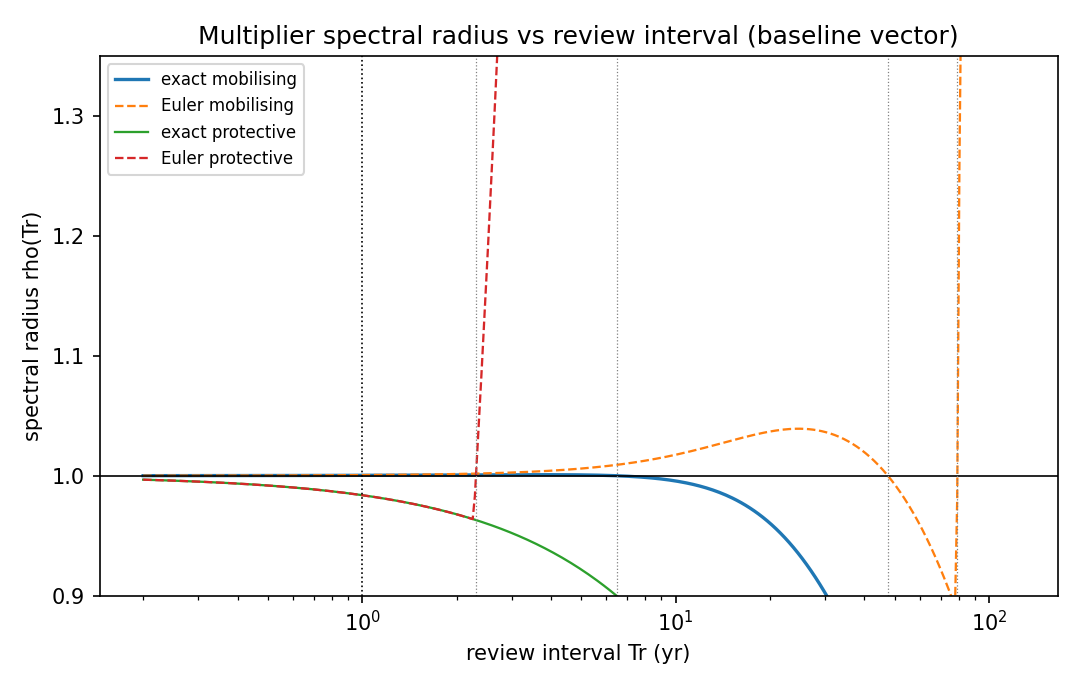
\includegraphics[width=0.9\linewidth]{figs_p5/fig_rho_scan_v39.png}
\caption{Spectral radius \(\rho(T_r)\) against review interval at the baseline parameter vector (Table 3) for the four update--channel combinations. Horizontal line: the unit circle; dotted verticals: the 6.501, 47.536, 79.143, and 2.306 yr crossings and the annual review (1 yr). The exact mobilising curve crosses once; the Euler mobilising curve reports two artefact crossings; the exact protective curve never reaches unity.}
\label{fig:rho-scan}
\end{figure}

\subsubsection{3.5 The selected 42-stock spectral
screen}\label{the-selected-42-stock-spectral-screen}

No stock in the screened cohort has a peak in the specified biomass target
bands meeting all robustness criteria. Baltic sprat, for example,
has a biomass coefficient of variation of 0.40, but its variation is
low-frequency and regime-dominated rather than a robust target-band
peak. The null carries a three-way restriction: it is not
proof of absence, not a comparison of controller signs, and not causal
evidence that annual review stabilises anything. On the stage-structured
review map (Section 3.3), annual-review stability at every tested response value is
consistent with this null; consistency is not a test. The institutional
reading is therefore limited: under this screen, target-band
cycles are not common in assessed-stock records, and any claim that
periodicity itself diagnoses an institutional feedback is unsupported by
this cohort. That null verdict is robust: an eleven-variant sensitivity
battery --- the AR(1) baseline plus ARMA(1,1), trend-stationary-no-detrend, circular block
bootstrap at three block lengths, Hodrick--Prescott-cycle and
first-difference pretreatments, and piecewise-AR(1) regime surrogates at
three break dates, each at the published 200-replicate, seed-7
resolution --- returns the BH-adjusted zero count in every variant
(smallest nominal \(p\) 0.0100, Hodrick--Prescott variant; details and
the resolution bound in Supplementary S9.1; the screen's restricted-result status is stated in Section 2.4).

The screen's zero count holds under exploratory alternative bands: a broad 2--10 yr band, management-cadence bands (1--3, 3--8, 8--20 yr), and an 8--80 yr effort-proxy band all return zero Benjamini--Hochberg-significant cells, with the effort-proxy band unresolvable (record span below three upper periods) on all 42 records (Supplementary S11). Figure~\ref{fig:screen} shows the baseline \(q\)-value distribution and per-stock null excess. Exploitation intensity carries no spectral excess once the ENSO confound is removed (Spearman 0.03 with Peru/Chile excluded, against 0.31 before; Supplementary S12). Across a 454-stock broader pool, the archived cohort median buffer-years (1.79) sits at the second percentile of resampled medians, independently re-executed (Supplementary S12).

\begin{figure}[htbp]
\centering
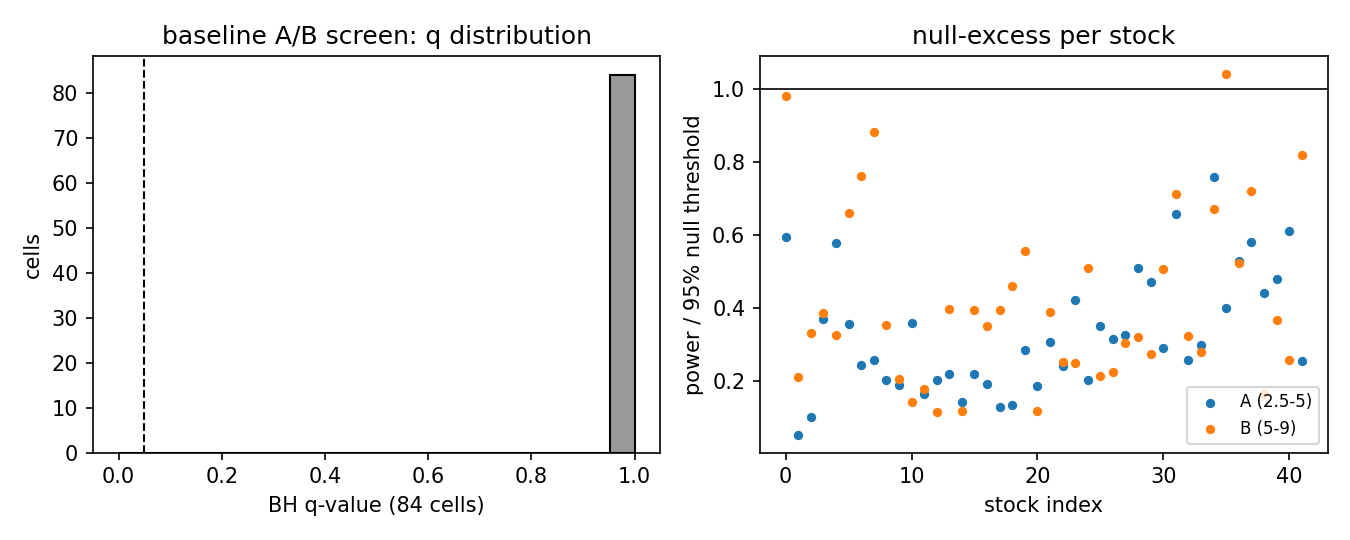
\includegraphics[width=0.9\linewidth]{figs_p5/fig_screen_v39.png}
\caption{Baseline screen diagnostics. Left: Benjamini--Hochberg \(q\)-values over the 84 target-band cells (dashed line: 0.05; no cell significant). Right: per-stock band power relative to the 95\% per-stock AR(1) threshold in bands A and B (horizontal line: unity).}
\label{fig:screen}
\end{figure}

\subsubsection{3.6 Power of the injected-signal
screen}\label{power-of-the-injected-signal-screen}

On 100--200 yr synthetic records, the sprat-class signal has estimated
power 1.0 at noise scale \(\sigma=0.1\) and approximately 0.24--0.58 at
\(\sigma=0.3\). The anchovy-class effort signal has power approximately
0.02--0.14 over the tested horizons and noise levels; its longer effort
peak and slow amplitude growth can offset its larger relative excursion.
These are conditional simulations: no minimum-power guarantee holds per
empirical stock, and the 100--200 yr horizons exceed many eligible
series. The anchovy-class null is consequently weakly informative under
this test, and the sprat-class result is informative only in
favourable noise and record-length regimes. The empirical screen is
therefore a selected-cohort consistency check and the baseline for a
prospective design, not a general test of the extractive mechanism. The sprat-class 1.0 at \(\sigma=0.1\) is trend detection (growth-transient run-up in the 30--120 yr band), not cycle detection, and is fragile at \(\sigma=0.3\).

The evidentiary separation is complete: the stage-dependent regions, noise
experiments, and power estimates do not establish population-wide
frequencies or policy effects and cannot be transferred to the
extractive hold-map controller or to protective control. The complementary prospective design is specified in Section 4.5 (detail in Supplementary S13.3).

\subsubsection{3.7 Structured case search: no qualifying cases}\label{the-zero-count-case-search}

No candidate satisfied all four criteria after primary-source and station-level review. The zero count is an evidential gap, not a disconfirmation: it records that no unconfounded oscillator was found, not that none exists. Bangkok (durably responsive institutional feedback: the groundwater-extraction control regime persisted across multiple review cycles rather than being a one-time cap or ban) and La Mancha Oriental (on the
stabilising side before its 2019--2023 extraction relapse) are the
closest cases. The unconfounded delay oscillators identified in
produced-capital systems (livestock and electricity-capacity cycles) do
not contain the autonomously regenerating stock the resource model
assumes. The per-system calculations use archived input series and are reported at that status in the
Supplementary material (S4); three groups illustrate the screening logic.

Sheridan-6 groundwater (hydrological driver without a feedback rule) and Icelandic cod and haddock under harvest-control rules (rule present, no review-cycle identification) illustrate the confound patterns at case level (Supplementary S4). The four-state prediction is the stage-structured review map's closed loop of four state components (adults \(A\), juveniles \(J\), memory signal \(Z\), held effort \(E\)), whose slow-stock class carries the centuries-scale dominant timescales of Section 3.3.

Peruvian anchoveta provides a further discriminator: a robust 3.7 yr catch periodicity with ENSO as candidate driver, evidence of shared periodicity rather than an identified mechanism (Supplementary S4 for the battery, multiplicity family, and confirmatory tests). The subannual review regime lies below the anchovy-class review-interval response region, so the unclassified controller prevents that comparison from testing the mechanism. The 3.7 yr catch periodicity is not a review interval.

Two structural hypotheses may help explain the zero count. The long
records needed to test the claim exist primarily for visible crises, and
visibility is correlated with a fast non-institutional driver. And on
the continuous-delay parameterisation that produces the instability
window (\(rg \approx 1.5\)--\(1.6\)) the predicted period is centuries
--- longer than any institution has held a fixed response rule --- while
the 3--12 yr windows belong to the stage-structured map. The two period
scales are properties of different operators and should not be read as
one prediction. The visible-record pattern --- long series repeatedly associated
with climate variability, cohort effects, infrastructure changes, or
emergency interventions --- suggests, without establishing, a selection
mechanism in which systems receive intensive monitoring after complex
crises; no causal identification of selection bias is claimed.

One documented system sits at the window's edge rather than inside it: the spruce budworm 30--40 yr outbreak cycle is endogenous predator--prey outbreak dynamics rather than institutionally driven (Supplementary S4 for the rate mapping and window comparison). The system corroborates the mechanism class, not the institutional claim.

\subsubsection{3.8 The northern cod two-window
split}\label{the-northern-cod-two-window-split}

The case's positive content is a descriptive partition, offered as a consistency check of the assessment-window mechanics rather than an empirical rejection of scalar autonomous or single-driver dynamics. \textbf{The
data split the phenomenon into two events --- the crash
interpretation is formulation-dependent, and the post-collapse dynamics
expose a second identification problem not resolved by the
mortality-allocation comparison. The split is the positive content, not
a new mechanism.}

The crash window (1991--1995) is documented by the assessment table (DFO
CSAS SAR 2016/026, Table A2; Table 2): spawning stock biomass falls from
735 to 10 kt across the five calendar years 1991--1995 while estimated
natural mortality reaches 2.2--2.6 yr\(^{-1}\), roughly ten times
pre-collapse levels (the pre-collapse reference period, estimator, and
uncertainty interval for this ratio are documented with the assessment
table; Table 2 begins in 1991). The displayed values are
rounded values from the assessment table . The
interpretation of the crash is a formulation attribution, not a causal
claim. The NCAM M-shift formulation allocates most estimated mortality
to natural death, and NCAM's \(M\) is an estimated unobserved-death
component conditional on model structure --- assessment-framework
proceedings explicitly caution that unreported fishing deaths may enter
de-facto \(M\) (Cadigan, 2016). The constrained-M formulation attributes
the crash to unreported catch. The constrained-M quantities are unreproduced (Supplementary S13.2 for the quantities and reproduction requirements): they are listed as open problems and stated here as hypotheses, not results.

\textbf{Table 2.} Northern cod spawning stock biomass (SSB) and
estimated instantaneous natural mortality (\(M\)) from DFO CSAS SAR
2016/026 (Table A2, NCAM M-shift formulation), rounded from the
assessment table. The survival column \(\exp(-M)\) is a transformation
of the reported \(M\) --- annual survival conditional on the estimated
natural-mortality component alone, since fishing mortality and other
modelled removals also apply --- not an independently observed survival
series.

\begin{longtable}[]{@{}llll@{}}
\toprule\noalign{}
Year & SSB (kt) & \(M\) (yr\(^{-1}\)) & \(\exp(-M)\) \\
\midrule\noalign{}
\endhead
\bottomrule\noalign{}
\endlastfoot
1991 & 735 & 1.002 & 0.367 \\
1992 & 382 & 2.214 & 0.109 \\
1993 & 101 & 2.575 & 0.076 \\
1994 & 31 & 2.331 & 0.097 \\
1995 & 10 & 0.288 & 0.750 \\
1996 & 16.05 & 0.341 & 0.711 \\
2000 & 34.42 & 0.717 & 0.488 \\
2004 & 20.07 & 0.362 & 0.696 \\
2005 & 25.18 & 0.288 & 0.750 \\
2010 & 96.91 & 0.696 & 0.499 \\
2015 & 298.65 & 0.278 & 0.757 \\
\end{longtable}

The non-recovery window is the second event. After the moratorium, the series both rises and falls across tens of thousands of tonnes (Table 2; the full annual record with uncertainty intervals is the assessment table). The phase-line obstruction of Section 2.7 applies as
a model-class diagnostic (not an empirical rejection of scalar autonomous models for northern cod): an error-free trajectory with repeated
direction reversals cannot arise from a fixed scalar autonomous model
with constant removals. The assessment record does not satisfy the
diagnostic's two conditions --- the SSB series is an assessment estimate
rather than an exact trajectory, and removals were not fixed through the
window --- so the proposition is a statement about model adequacy for
this class, not a direct empirical rejection. Two scope statements
govern the result. The reliable contradiction is repeated direction
reversal: convergence toward \(K\) can be arbitrarily slow near
degeneracy, so failure to reach an unspecified biomass by an unspecified
deadline is not a contradiction. And the obstruction must be separated
from rejection under measurement error, process noise, age structure,
migration, time-varying mortality, and state-space observation models
--- the incompatibility is a property of the exact trajectory class,
nothing broader.

The subsequent record does not close the second window. Rose (2026),
comparing two surplus-production reconstructions spanning 1983--2023
(Rose and Walters, 2019; DFO, 2024), documents that surplus production
and stock growth stalled after 2015, with some years negative, and that
the stall-point biomass remains controversial. Structural-equation
analyses in the same review attribute the production deficit to capelin
limitation and harp seal predation rather than fishing alone. For the
present analysis the key point is the persistence of the
non-recovery: a decade after the rebound reported by Rose and Rowe
(2015), the post-2015 production stall is inconsistent with the simplest
fixed-parameter surplus-production interpretation considered here, which
is precisely what the split's second window --- a second identification
problem not resolved by the mortality-allocation comparison --- states. Read through Lemma 2.2(ii), the seal-predation attribution carries a directional consequence: to the extent predation acts as additional mortality on the stock, the effective threshold facing recovery lies above \(\mathfrak s\), so predation raises the threshold for re-establishment rather than merely slowing convergence. No predation-mortality rate is estimated here; the lemma is used for the direction of the effect, not its magnitude.

The ecosystem context (Supplementary S5) is background only: the harp seal increase and capelin decline in the mass-balance record (Tam and Bundy, 2019) are descriptive inputs, not causal tests.

Figure~\ref{fig:cod} plots the Table-2 SSB and mortality series against the two windows.

\begin{figure}[htbp]
\centering
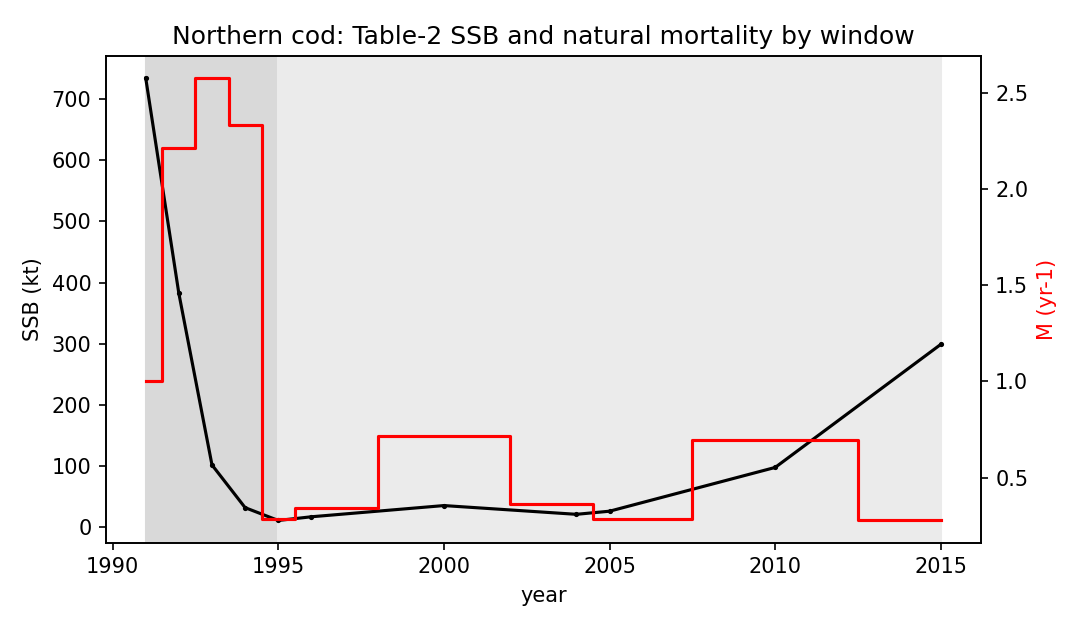
\includegraphics[width=0.9\linewidth]{figs_p5/fig_cod_v39.png}
\caption{Northern cod Table-2 series by window. Black: spawning stock biomass; red steps: instantaneous natural mortality; shaded: the crash (1991--1995) and non-recovery (1995--2015) windows.}
\label{fig:cod}
\end{figure}

Table 5 collects the Section 3 results with their evidential status; Supplementary S1 is the complete inventory.

\textbf{Table 5.} Results at a glance: each Section 3 result with its evidential status.

\begin{longtable}[]{@{}
  >{\raggedright\arraybackslash}p{(\columnwidth - 2\tabcolsep) * \real{0.5000}}
  >{\raggedright\arraybackslash}p{(\columnwidth - 2\tabcolsep) * \real{0.5000}}@{}}
\toprule\noalign{}
\endhead
\bottomrule\noalign{}
\endlastfoot
Forward invariance (Section 3.1) & theorem \\
Rapid-review consistency (Section 3.2) & conditional theorem (finite horizons) \\
Response regions (Section 3.3) & archived records (provisional) \\
Crossing record; battery, F-grid, NS records (Section 3.4) & re-execution-verified computation; nominal-tier records (S11) \\
Screen null; alternative bands; F-excess; ADH (Section 3.5) & re-execution-verified zero count; nominal-tier records (S9.1, S11, S12) \\
Power analysis (Section 3.6) & independently re-executed computation \\
Case search (Section 3.7) & executed search (evidential gap, not disconfirmation) \\
Cod two-window split (Section 3.8) & descriptive partition; hypotheses, not results \\
\end{longtable}

\subsection{4 Discussion}\label{discussion}

\subsubsection{4.1 Architecture substitution: what changes when the
operator
changes}\label{architecture-substitution-what-changes-when-the-operator-changes}

The operator-spectra results of Section 3.4 are the paper's core methodological finding. Stability windows are operator-specific: they do not transfer across review-map operators. The same feedback loop --- surplus production,
an institutional deficit signal, an effort law --- carries an archived,
unreproduced instability record near 3--4 yr of review under the
stage-structured map, convergence over a 1--20 yr grid under that map's
cod-class parameterisation, and instability at annual review with a
complex crossing near 6.5 yr under the exact logistic hold map (full
records, the Euler command-step artefact, and the \(q\)-sensitivity
caveat in Section 3.4 and its Reading; the plant--operator confound is
stated alongside and the operator effect is not claimed isolated).

The complete crossing record sharpens the operator finding: on one plant the exact and Euler updates disagree on the number and location of crossings (Section 3.4). The review cadence is a local spectral design parameter, and the
command step is a second, independent one. None of these statements can
be obtained from the continuous-delay equation, and none transfers to
it. Any empirical or theoretical claim about institutional feedback must
therefore state its operator: a stability window located under
continuous delay is not a prediction about an institution that reviews
periodically, and an annual-review result does not generalise to
multi-year plans. The governance architecture itself is a testable
component of the hypothesis, not a re-parameterisation detail.

\subsubsection{4.2 What the null does and does not
establish}\label{what-the-null-does-and-does-not-establish}

The 42-stock screen returns a spectral null, and its value lies in what
it refutes: the claim, implicit in treating periodicity as evidence,
that robust target-band cycles are common in assessed-stock records. It
does not establish the contrary. With anchovy-class power between 0.02
and 0.14 across tested noise and record-length regimes, the screen
cannot adjudicate the extractive mechanism for that class; the
sprat-class result is informative only in favourable regimes; and no
screen of retrospective series can compare controller signs, because the
sign is not in the data. This is the same null discipline that the
skeptical re-analysis of the Russell Cycle applied to climate-forced
cycles (McManus, Licandro, and Coombs, 2016), transferred to
governance-feedback claims: a diagnostic is not a causal claim, and no
accumulation of diagnostics converts to causal evidence.

\subsubsection{4.3 The cod case at its exact
status}\label{the-cod-case-at-its-exact-status}

The cod case contributes a descriptive partition, not a mechanism:
crash-window mortality is formulation-dependent (Section 3.8), and the
post-collapse record is not resolved by either mortality-allocation
formulation, with the post-2015 production stall persisting under
independent reconstructions (Rose, 2026). The obstruction mathematics
applies within the scope stated in Sections 3.8 and 4.7(vii). What the
case supplies is a falsification benchmark: a well-documented
collapse-and-stall record against which prospective designs can be
powered and scored.

\subsubsection{4.4 A falsification standard for institutional-feedback
claims}\label{a-falsification-standard-for-institutional-feedback-claims}

The model family gains empirical content by specifying the outcomes that
count against its mechanism and parameterisation. Five outcomes:

\begin{enumerate}
\def\labelenumi{\arabic{enumi}.}
\tightlist
\item
  If independently measured implementation and deployment lags do not
  covary with the instability bands predicted under fitted resource
  parameters, the quantitative delay claim is weakened.
\item
  If an observed oscillation remains after climate, cohort, and regime
  forcing are modelled, but its phase relation between decline signal,
  effort, and biomass contradicts the controller's causal ordering, the
  mechanism is rejected for that case.
\item
  If sampled-data analysis removes a continuous-delay band under
  realistic review rules, the continuous model cannot be used for that
  institution.
\item
  If a protective controller dominates the extractive controller across
  uncertainty without inducing the claimed volatility, no
  anti-regulation conclusion may be drawn.
\item
  If realistic record lengths have low power for the predicted signal, field spectral nulls cannot adjudicate the mechanism; prospective or experimental evidence is required. The Icelandic cod case illustrates the bind: its post-1995 variability (coefficient of variation 0.37--0.39; no dominant spectral peak, Supplementary S11) overlaps the continuous-delay band (9.9--20.3 yr) in timescale yet carries no institutional signature, because a competing environmental driver is empirically supported for the same outcome (criterion (iii); Supplementary S4).
\end{enumerate}

\subsubsection{4.5 Prospective designs}\label{prospective-designs}

The retrospective evidence does not identify the institutional
mechanism; the constructive content of this paper is the programme that
could. Retrospective evidence can still discipline the mechanism where a prespecified contrast exists: the \(T_r\)-ranked cross-sectional test across the 42-stock cohort is executed in Supplementary S10 and returns a controlled null --- no window-approach gradient, with \(T_r \approx 1\) dormancy holding at 0/42 and 1/42 flags in the two bands. Five designs are specified as preregistration targets; none has been executed, and each is intended for preregistration before outcome
inspection --- no registration identifier or archived protocol exists
yet, and none is claimed.

\textbf{Governance-event panels.} For each resource--jurisdiction unit, a source-linked event record dates each stage from raw observation to ecological response, with date uncertainty kept distinct rather than collapsed to one lag (full specification in Supplementary S13.3). The cod case supplies two dated decision events --- the moratorium announcement of 2 July 1992 and the reopening of 26 June 2024 with an 18 kt total allowable catch --- with two negative constraints: no governance lead is inferred from annual biomass data, and a fast response does not establish adequacy.

\textbf{Quasi-experimental timing.} Event-study, difference-in-differences, synthetic-control, interrupted-time-series, or state-space intervention designs on schedule variation plausibly independent of the outcome innovation, with preregistered estimands (full specification in Supplementary S13.3). Two coding rules are binding: a change in implementation lag is not coded as a change in \(T_r\), and a nominal schedule change is not a treatment unless it changes a responsive decision opportunity.

\textbf{Out-of-sample mechanism comparison and the displacement
discipline.} Held-out comparison across environmental-forcing, cohort-resonance, institutional-delay (specified controller sign), combined, and null time-series models, with frozen splits and declared outcomes (full specification in Supplementary S13.3). The displacement rule: a delay explanation is weakened when it cannot reproduce the pre-registered phase ordering, and displaced when a competitor predicts the held-out observations better.

\textbf{Controlled and randomized human-in-the-loop experiments.} Randomised review cadence and feedback timing or sign in a common simulated renewable-resource environment, with the gain--phase signature as the diagnostic target (full specification in Supplementary S13.3). The randomisation described is a laboratory or advisory-interface design, not a field intervention on a live stock; mechanism-class precedent exists (Costantino, Cushing, Dennis, and Desharnais, 1995; Moxnes, 1998) but is not validation of the institutional equations.

\textbf{Closed-loop management strategy evaluation.} Policy comparison in a closed loop keeping six uncertainty classes distinct (the management-procedure tradition: Punt and Donovan, 2007), crossing review timing, delays, controller sign, observation error, parameter draws, operating-model class, and process-noise regime (full specification in Supplementary S13.3). At minimum, responsive extractive, responsive protective, and fixed-plan controllers are compared; a conclusion that compares only two review intervals inside the extractive class cannot be generalised to governance as a whole. Three wider empirical hypotheses of the programme's general theory --- observation aggregation, governance phase ordering, and substitution certificate --- are adopted here only as motivation, and otherwise explicitly deferred: governance phase ordering supplies the gain--phase diagnostic target the designs above inherit, while testing any of the three requires prospective, adequately powered designs this paper specifies but does not execute.

\subsubsection{4.6 Distributive constraints where
reproducible}\label{distributive-constraints-where-reproducible}

The social side of the cod case is presented at measurement level (Appendix B): the constituency-definition
mismatch table (licence holders against census-subdivision residents;
fishing income against all-resident sector income; the unspecified
floor), the Statistics Canada community-level series (tables
38-10-0167-01 and 38-10-0168-01), the measured-floor construction
\((I_k, c_k)\) with its componentwise non-decline rule, and the admitted
world-hook instruments are given in Appendix B, with the full
instrument detail and the unreproduced pipeline register in the
Supplementary material (S6). What the case does not measure is the
point: no licence-holder panel exists, the community series is not
one, and no measured floor is operational --- the distributive
constraints remain stated rather than resolved (Section 4.7 (viii)).

\subsubsection{4.7 Limitations}\label{limitations}

\begin{enumerate}
\def\labelenumi{(\roman{enumi})}
\tightlist
\item Diagnostics are not causal claims: the spectral null, the response regions, the power values, the case calculations, and the cod split carry their stated types and no more.
\item The stage-structured response regions are exploratory finite-grid, trajectory-classified records pending complete stage registration and multiplier analysis; the logistic hold-map multiplier record is complete (Section 3.4), and the stage operator's multiplier and trajectory record is supplied by the reconstruction of Section 3.4 --- a newly specified object whose comparison with the archived windows is a consistency check, not a validation. No Poincar\'e-map multiplier classification is claimed for the archived stage-output values, and they are not reproducible numerical propositions until the original computational record is attached. The effort scale is uncalibrated: results are reported at imported catchability values, and reparameterising the controller in fishing mortality (\(F = qE\)) is the stated next step for the stage operator.
\item The two review-map operators are distinct: statements computed on the hold map, on the stage-structured map, and on the continuous-delay equation do not transfer to one another.
\item The screen is a selected-cohort consistency check whose power is high only in favourable noise and record-length regimes; the null is not proof of absence and adjudicates nothing about controller sign; the AR(1) null may understate low-frequency power. The eleven-variant battery of Supplementary S9.1 holds the zero count under ARMA(1,1), trend-stationary, block-bootstrap, detrending, and regime-shift nulls; the remaining masked-peak risk runs via overestimated null power (unmodelled observation-error or retrospective-bias variance raising the threshold), not the underestimation above.
\item The structured case search does not independently disconfirm the mechanism: finding no eligible cases under these criteria is not evidence against it.
\item The cod case establishes a descriptive partition, and no mechanism is identified.
\item The obstruction mathematics concerns exact trajectories of the fixed-parameter, fixed-removals autonomous class and is not a rejection under measurement error, process noise, age structure, migration, time-varying mortality, or state-space observation models.
\item The social object is not operationalised: the human series is not assembled, the normative floors are unoperationalised, and documenting the gap is the finding.
\item The prospective designs are preregistration targets, not executed studies, and they do not retroactively change the status of the retrospective results.
\end{enumerate}

\subsubsection{4.8 Design principles for the governance clock}\label{design-principles}

The results support four design principles for the decision clock (Box 2).

\textbf{Box 2. Design principles for the governance clock.}

\begin{longtable}[]{@{}
  >{\raggedright\arraybackslash}p{(\columnwidth - 4\tabcolsep) * \real{0.3333}}
  >{\raggedright\arraybackslash}p{(\columnwidth - 4\tabcolsep) * \real{0.6667}}@{}}
\toprule\noalign{}
\begin{minipage}[b]{\linewidth}\raggedright
Principle
\end{minipage} & \begin{minipage}[b]{\linewidth}\raggedright
Content
\end{minipage} \\
\midrule\noalign{}
\endhead
\bottomrule\noalign{}
\endlastfoot
Treat timing as a control variable & The review interval is optimised alongside harvest limits in management strategy evaluation; annual review is not assumed stabilising. \\
Match the rule to the clock & Protective rules tolerate institutional rigidity; extractive rules require frequent review to contain destabilisation. \\
Decouple observation from decision & High-frequency monitoring does not require high-frequency revision; multi-year plans are stable under protective rules. \\
Design for structural breaks & Scheduled review is paired with asynchronous emergency triggers (circuit breakers) that bypass the review clock during regime shifts. \\
\end{longtable}

\textbf{Implications for management design.} Eight implications follow for review-interval choice. \begin{enumerate} \def\labelenumi{(\arabic{enumi})} \tightlist \item The review interval is a control variable: stability is computed per interval, not per loop (Section 3.4). \item Annual review is not automatically stabilising: the baseline annual verdict is unstable with a near-unit-circle margin (Section 3.4). \item Protective rules are more robust across review intervals than extractive rules: the exact protective map is stable at every tested interval (Section 3.4). \item Fixed and responsive plans are not equivalent instruments: a held multi-year command and an annually revised rule are different operators (Sections 2.6 and 4.4). \item Emergency triggers are modelled separately from scheduled reviews: structural breaks between reviews are invisible to the fixed clock (Sections 3.8 and 4.5). \item Management strategy evaluation treats the review interval as an explicit factor alongside the control rule (Section 4.5). \item Spectral periodicity is not evidence of institutional cycles: the screen's null carries no controller-sign information (Sections 3.5--3.7). \item Observation, assessment, decision, deployment, and response lags are not collapsed into one governance lag (Section 2.1). \end{enumerate}

Beyond fisheries, the framework is reusable as a modelling discipline: it answers how periodic governance should be represented in ecological models, how the stages of the advice chain should be kept distinct, and how modellers can test whether a stability claim survives a change of decision operator.

The logistic core is illustrative; the structural results are the operator-dependence of the stability verdict, the finite-horizon scope of the rapid-review limit, and the non-equivalence of one-step and exact updates as a caution within the studied class.

Sample-and-hold architectures beyond fisheries face the same clock-mismatch failure mode: five-yearly climate pledges held between global stocktakes (UNFCCC, 2015) align a political review clock with ecological and environmental clocks only by design, not by default.

\subsection{5 Conclusion}\label{conclusion}

Periodic review is the operating architecture of fisheries governance,
and it is not well represented by either of its standard formalisations.
The sample-and-hold model specified here makes the governance clock an
explicit object: seven time objects, a projected explicit controller,
and a spectrum computed per operator rather than per loop. Its empirical
layer contains one case whose
positive content is a descriptive split --- the northern cod two-window
partition --- and a falsification discipline for the rest: a selected-cohort
screen with no target-band discoveries and stated power, a zero-count
case search with its structural hypotheses, and a falsification standard
with five outcomes that count against the mechanism. The mechanism is
falsifiable, and the five prospective designs specify how it would be
falsified, comparatively supported, or left unresolved. Until those
designs are executed, the empirical layer stands as stated here: a
well-posed mechanism, an exploratory computational record, limited
screen power, a case search that does not disconfirm, and one descriptive split. The decision clock --- the timing and form of policy revision --- is therefore a design variable with stability consequences.

\subsection{Appendix A. Registration and reproducibility record
(consolidated)}\label{appendix-a.-registration-and-reproducibility-record-consolidated}

This appendix collects the registration and reproducibility requirements stated in Sections 2.2, 2.4, 2.5, 3.3, and 3.4. The convention: an analysis is pre-registered when its plan is dated and fixed before any run, as the stage-map reconstruction of Section 3.4 is; computational artifacts (solver configuration, seeds, identifiers, calibration records) are archived with the materials. The consolidated requirements:

\begin{itemize}
\tightlist
\item
  The solver configuration and initial histories are
  registration requirements; until that computational record is complete,
  the stage-output values carry provisional status (Sections 2.2 and
  3.3).
\item
  The RAM stock identifiers and the eligibility table are
  archived with the computational materials (Section 2.4).
\item
  The full null-calibration record --- AR(1) coefficient estimation,
  detrending inside each null replicate, missing-data treatment, and the
  number of Monte Carlo replicates --- is archived with the computational materials (Section 2.4).
\item
  The simulation code and seeds are archived with the computational materials
  (Section 2.5).
\end{itemize}

Two further consolidated records. First, the logistic-core parameter
vector (\(r\), \(K\), \(E_{\max}\), \(\delta_0\), \(Z_{\rm ref}\),
\(\Delta_{\rm ref}\), \(\tau_m\); \(\delta = \log 2/10\) is stated in
Section 2.1) and the linearised fixed point \((N^*, E^*, Z^*)\) with its
interiority to the nonsmooth regions of \(\Phi_k\) and
\(\Pi_{[0,E_{\max}]}\) are printed in Table 3, with the code constants
block pinned per row; the monodromy's numerical construction and the
continuous eigenvalue \(\lambda\) and crossing angle \(\theta\) of
Section 3.4's records remain part of the computational record. Second, the Data
availability statement records the deposit status of the same
requirements (including the reconstruction's dated plan, campaign code,
and output tables); the prospective designs of Section 4.5 remain
preregistration targets with no registration identifier or archived
protocol. The full discharge register is Supplementary S8.

\textbf{Table 3.} Parameter values for the
logistic hold-map core and the stage-structured reconstruction. No value here is newly computed except the linearised-gains, crossing-angle, eigenvalue, and solver rows, which are computed in Supplementary S11; the baseline-core vector is printed here, with the code constants block pinned per row, and values not stated remain in
the computational record (this appendix). Time is in years; biomass, effort, and signal scales are bare model units (\(K\), \(E_{\max}\), \(Z_{\rm ref}\), and \(\Delta_{\rm ref}\) set the scales).

\begin{longtable}[]{@{}
  >{\raggedright\arraybackslash}p{(\columnwidth - 6\tabcolsep) * \real{0.2500}}
  >{\raggedright\arraybackslash}p{(\columnwidth - 6\tabcolsep) * \real{0.2500}}
  >{\raggedright\arraybackslash}p{(\columnwidth - 6\tabcolsep) * \real{0.2500}}
  >{\raggedright\arraybackslash}p{(\columnwidth - 6\tabcolsep) * \real{0.2500}}@{}}
\toprule\noalign{}
\begin{minipage}[b]{\linewidth}\raggedright
Object
\end{minipage} & \begin{minipage}[b]{\linewidth}\raggedright
Parameter
\end{minipage} & \begin{minipage}[b]{\linewidth}\raggedright
Value as stated
\end{minipage} & \begin{minipage}[b]{\linewidth}\raggedright
Stated at
\end{minipage} \\
\midrule\noalign{}
\endhead
\bottomrule\noalign{}
\endlastfoot
Logistic hold-map core & catchability \(q\) & 0.001 & Section 3.4 (stage Plant paragraph, as the hold-map core's value) \\
Logistic hold-map core & softplus sharpness \(k\) & 10 & Section 3.4
(Plant paragraph) \\
Logistic hold-map core & effort-response coefficient \(\eta\) & 0.914 & This table; constants block \texttt{droop\_test.py} L49--58 @ 24c980cd; inherited illustrative baseline (Candidate-A value from the companion delay study, whose institutional coefficients are explicitly uncalibrated: Abaee, 2026); the delay-Hopf window opens between \(\eta = 0.5\) and \(0.7\) and the \(r = 0.02\) inclusion threshold sits at \(\eta^* \approx 0.85\), so 0.914 is neither threshold (basis runs deposited; Supplementary S9.2) \\
Logistic hold-map core & growth rate \(r\) (yr\(^{-1}\)) & 0.02
(validation argument) & This table; constants block
\texttt{droop\_test.py} L49--58 @ 24c980cd \\
Logistic hold-map core & carrying capacity \(K\) & 100 & This table;
constants block \texttt{droop\_test.py} L49--58 @ 24c980cd \\
Logistic hold-map core & effort ceiling \(E_{\max}\) & 30 & This
table; constants block \texttt{droop\_test.py} L49--58 @ 24c980cd \\
Logistic hold-map core & effort-law gain \(\delta_0\) & 0.01 & This
table; constants block \texttt{droop\_test.py} L49--58 @ 24c980cd \\
Logistic hold-map core & reference deficit \(Z_{\rm ref}\) & 1 & This
table; constants block \texttt{droop\_test.py} L49--58 @ 24c980cd \\
Logistic hold-map core & reference scale \(\Delta_{\rm ref}\) & 1 &
This table; constants block \texttt{droop\_test.py} L49--58 @ 24c980cd \\
Logistic hold-map core & memory timescale \(\tau_m\) (yr) & 5 & This
table; constants block \texttt{droop\_test.py} L49--58 @ 24c980cd \\
Logistic hold-map core & memory shift \(\delta\) & \(\log 2/10 \approx 0.069\) (equilibrium memory level) & Section 2.1 \\
Logistic hold-map core & linearised fixed point \((N^*, E^*, Z^*)\);
interiority & \((89.55188, \delta, 2.08962)\); \(E^* \in (0,
E_{\max})\), \(\Phi_k(0) = \delta\), \(sp_k'(0) = 1/2\) & This table;
equilibrium routine \texttt{base\_equilibrium},
\texttt{droop\_test.py} L86--93 @ 24c980cd; closed form in Supplementary S2.3 \\
Logistic hold-map core & crossing record & 47.536, 79.143, 2.306, 6.501
yr; \(\rho\) = 1.00035, 1.00055, 0.9838, 0.9967 & Section 3.4 \\
Logistic hold-map core & scan construction & 200,001-point scan with
bisection over \([0.2, 200]\) yr & Section 3.4 \\
Logistic hold-map core & linearised mobilising gains \((C_E, C_Z)\) & \((-0.059518, +1.785019)\) & Supplementary S11 (sensitivity battery) \\
Logistic hold-map core & crossing angle \(\theta_0\) (exact map, 6.501 yr) & 0.175494 rad & Supplementary S11 \\
Logistic hold-map core & continuous eigenvalues \(\lambda\) (undelayed loop) & \(-0.278147\), \(+0.000360\pm0.027683i\) & Supplementary S11 \\
Logistic hold-map core & derivative construction & closed-form monodromy (no finite differences) & Section 3.4 \\
Logistic hold-map core & solver; precision; grid check & matrix exponential (\texttt{expm}); IEEE-754 double; 2k/20k/200k scans identical; 50-digit certificate (S12) & Supplementary S11 \\
Stage reconstruction & class natural mortality \(M\) and recruitment
delay \(\tau\) & anchovy (0.90, 1), sprat (0.40, 2), cod (0.20, 5),
slow-stock (0.045, 25) yr & Section 3.4 (Plant paragraph, with
sources) \\
Stage reconstruction & steepness \(h\) & 0.75; sensitivity
layer \(\{0.6, 0.9\}\) & Section 3.4 \\
Stage reconstruction & scale and survival & \(A_0 = 100\);
\(s_A = s_J = e^{-M}\); \(\beta = (c-1)/A_0\),
\(\alpha = c(1-s_A)/s_J\), \(c = 4h/(1-h)\) & Section 3.4 \\
Stage reconstruction & catchability \(q\) & 0.001; sensitivity
0.1 & Section 3.4 \\
Stage reconstruction & softplus sharpness \(k\) & 10 & Section 3.4 \\
Stage reconstruction & derivative construction & central finite
differences, step \(10^{-6}\), chain-rule cross-check to \(10^{-4}\) &
Section 3.4 \\
Stage reconstruction & scan grid & \(T_r \in \{1,\ldots,50\}\) yr at
annual internal steps & Section 3.4 \\
Stage reconstruction & trajectory classification & 2000 review-steps,
tail 500, relative tail standard-deviation thresholds 2\% and 0.1\%;
initial condition at the unfished plant equilibrium, memory filled,
effort at half the equilibrium & Section 3.4 \\
\end{longtable}

\textbf{Table 4.} Notation: every symbol with its definition site. No
row introduces a symbol; rows without a site would be gaps, and all
rows resolve.

\begin{longtable}[]{@{}
  >{\raggedright\arraybackslash}p{(\columnwidth - 4\tabcolsep) * \real{0.2500}}
  >{\raggedright\arraybackslash}p{(\columnwidth - 4\tabcolsep) * \real{0.4500}}
  >{\raggedright\arraybackslash}p{(\columnwidth - 4\tabcolsep) * \real{0.3000}}@{}}
\toprule\noalign{}
\begin{minipage}[b]{\linewidth}\raggedright
Symbol
\end{minipage} & \begin{minipage}[b]{\linewidth}\raggedright
Meaning
\end{minipage} & \begin{minipage}[b]{\linewidth}\raggedright
Defined at
\end{minipage} \\
\midrule\noalign{}
\endhead
\bottomrule\noalign{}
\endlastfoot
\(N\) & resource stock & Section 2.1 \\
\(Z\) & institutional deficit signal & Section 2.1 \\
\(E\) & extraction effort & Section 2.1 \\
\(\mathcal P_{T_r}\) & review Poincar\'e map (sampled flow at review
instants) & Section 2.1 \\
\(D\mathcal P_{T_r}(X^*)\) & monodromy matrix (Jacobian at the fixed
point) & Section 2.1 \\
\(\Pi\) & projection onto \([0,E_{\max}]\) & Section 2.1 \\
\(\Phi\), \(\Phi_k\) & signal map; softplus realisation (shift
\(\delta\), sharpness \(k\)) & Section 2.1 \\
\(\delta\); \(\delta_0\) & equilibrium memory level \(\log 2/10\);
effort-law gain (unrelated) & Section 2.1 \\
\(F_B\); \(F_B^{\rm prot}\) & extractive effort law; protective
comparator & Section 2.1 \\
\(\mathcal A_n\); \(\mathcal O\) & assessment operator; observation
operator & Section 2.1 \\
\(S(\cdot)\); \(S\) & surplus production (control sections); spawning
stock biomass (cod sections, Table 2) & Section 2.1; Sections 2.7, 3.8 \\
\(g\) & maturation delay (delayed-recruitment parameterisation) &
Section 3.3 \\
\(C_E\), \(C_Z\) & linearised effort-law coefficients (per channel; protective values in Section 2.1) & Section 3.4 (Abaee,
2026, equation~(3)) \\
\(A\), \(J\), \(Z\), \(E\) & four-state loop: adults, juveniles, memory
signal, held effort & Section 3.7 \\
\(\mathfrak s\), \(K\), \(C(t)\), \(M\), \(M_x\), \(F\) & cod case: unstable
threshold, unexploited capacity, removals, natural mortality, extra mortality, fishing
mortality & Sections 2.7, 3.8; Table 2 \\
\end{longtable}

\subsection{Appendix B. Distributive constraints where reproducible}
\label{appendix-b.-distributive-constraints-where-reproducible}

Where the social side of the cod case can be presented, it is presented at
measurement level. The worst-off relevant population is a modelling
choice --- a named constituency --- and the candidate
constituency for 2J3KL is the registered inshore harvesters and licence
holders. The measurement record against that candidate is the following
mismatch table, each row stated rather than resolved:

\begin{longtable}[]{@{}
  >{\raggedright\arraybackslash}p{(\columnwidth - 8\tabcolsep) * \real{0.2000}}
  >{\raggedright\arraybackslash}p{(\columnwidth - 8\tabcolsep) * \real{0.2000}}
  >{\raggedright\arraybackslash}p{(\columnwidth - 8\tabcolsep) * \real{0.2000}}
  >{\raggedright\arraybackslash}p{(\columnwidth - 8\tabcolsep) * \real{0.2000}}
  >{\raggedright\arraybackslash}p{(\columnwidth - 8\tabcolsep) * \real{0.2000}}@{}}
\toprule\noalign{}
\begin{minipage}[b]{\linewidth}\raggedright
Object
\end{minipage} & \begin{minipage}[b]{\linewidth}\raggedright
Candidate definition
\end{minipage} & \begin{minipage}[b]{\linewidth}\raggedright
Available measure
\end{minipage} & \begin{minipage}[b]{\linewidth}\raggedright
Mismatch
\end{minipage} & \begin{minipage}[b]{\linewidth}\raggedright
Required data
\end{minipage} \\
\midrule\noalign{}
\endhead
\bottomrule\noalign{}
\endlastfoot
Population & registered licence holders & census-subdivision residents &
not the same population & licence microdata \\
Income & fishing income & all-resident sector income (incl.~aquaculture,
processing) & includes non-fishing income & administrative income \\
Floor & specified cutoff \((I_k, c_k)\) & none operational & not specified
& specified instrument and cutoff \\
\end{longtable}

The available community-level series (Statistics Canada tables
38-10-0167-01 and 38-10-0168-01; mean income from fishing falling from
32.2\% to 25.6\% across 43 fishing-dependent census subdivisions,
2016--2021) is all-resident employment income including aquaculture and
processing. The constituency must therefore either be redefined to the
census-subdivision populations, or licence-holder microdata or
administrative data must be obtained --- the community table is not a
licence-holder panel. A measured floor is a pair \((I_k,c_k)\) --- an
instrument and a cutoff --- a measurement object distinct from the norm
that motivates it, and the componentwise rule is that the arrangement
fails as soon as any measured margin \(m_k(G,t)=I_k(G,t)-c_k\) is
negative; the conjunction admits no compensatory master scalar.
Non-decline is a normative rule, not automatically an empirically
justified floor: baseline, cohort, inflation and purchasing-power
treatment, uncertainty, attrition, acceptable variation, authority, and
structural diversification all must be specified before a floor
measures anything. The instruments admitted as world-hooks (the global
Multidimensional Poverty Index of Alkire and Foster, 2011; the World
Bank Poverty and Inequality Platform) carry release and vintage locks,
and what they cannot capture --- who pays for persistence, who may use
remaining variety, whose knowledge counts, future persons --- is stated
as a boundary and left open rather than filled with a scalar score. The
full instrument detail and the unreproduced pipeline register are in the
Supplementary material (S6).

\subsection{References}\label{references}

Abaee, A. 2026. Delay-induced regime change in harvested stocks: the
mobilising and protective channels of institutional feedback, and the
review interval as control. Zenodo.
https://doi.org/10.5281/zenodo.22554217.

Alkire, S., and Foster, J. 2011. Counting and multidimensional poverty
measurement. Journal of Public Economics, 95: 476--487.

Ashwin, P., Wieczorek, S., Vitolo, R., and Cox, P. 2012. Tipping points
in open systems: bifurcation, noise-induced and rate-dependent examples
in the climate system. Philosophical Transactions of the Royal Society
A, 370: 1166--1184.


Benjamini, Y., and Hochberg, Y. 1995. Controlling the false discovery
rate: a practical and powerful approach to multiple testing. Journal of
the Royal Statistical Society B, 57: 289--300.

Benjamini, Y., and
Yekutieli, D. 2001. The control of the false discovery rate in multiple
testing under dependency. Journal of the Royal Statistical Society B,
63: 425--441.

Branch, T. A. 2001. A review of orange roughy Hoplostethus atlanticus
fisheries, estimation methods, biology and stock structure. South
African Journal of Marine Science, 23: 181--203.

Cadigan, N. G. 2016. A state-space stock assessment model for northern
cod, including under-reported catches and variable natural mortality
rates. Canadian Journal of Fisheries and Aquatic Sciences, 73: 296--308.

Ch\'avez, F. P., Ryan, J., Lluch-Cota, S. E., and Niquen, M. 2003. From
anchovies to sardines and back: multidecadal change in the Pacific
Ocean. Science, 299: 217--221.

Cohen, J. 1988. Statistical Power Analysis for the Behavioral Sciences,
2nd edn. Lawrence Erlbaum, Hillsdale, NJ.

Costantino, R. F., Cushing, J. M., Dennis, B., and Desharnais, R. A.
1995. Experimentally induced transitions in the dynamic behaviour of
insect populations. Nature, 375: 227--230.

DFO. 2011. Recovery potential assessment for the Newfoundland and
Labrador Designatable Unit (NAFO Divs. 2GHJ, 3KLNO) of Atlantic Cod. DFO
Canadian Science Advisory Secretariat Science Advisory Report 2011/037.

DFO. 2016. Stock Assessment of Northern cod (NAFO Divs. 2J3KL) in 2016.
DFO Canadian Science Advisory Secretariat Science Advisory Report
2016/026.

DFO. 2022. Stock Assessment of Northern cod (NAFO Divs. 2J3KL) in 2022.
DFO Canadian Science Advisory Secretariat Science Advisory Report
2022/041.

DFO. 2024. NAFO Divisions 2J3KL Northern cod (Gadus morhua) stock
assessment to 2024. DFO Canadian Science Advisory Secretariat Science
Advisory Report.

Forssell, U., and Ljung, L. 1999. Closed-loop identification revisited.
Automatica, 35: 1215--1241.

Gurney, W. S. C., Blythe, S. P., and Nisbet, R. M. 1980. Nicholson's
blowflies revisited. Nature, 287: 17--21.

Guti\'errez, D., Sifeddine, A., Field, D. B., Ortlieb, L., Vargas, G.,
Ch\'avez, F. P., Velazco, F., Ferreira, V., Tapia, P., Salvatteci, R.,
Boucher, H., Morales, M. C., Vald\'es, J., Reyss, J.-L., Campusano, A.,
Boussafir, M., Mandeng-Yogo, M., Garc\'ia, M., and Baumgartner, T. 2009.
Rapid reorganization in ocean biogeochemistry off Peru towards the end
of the Little Ice Age. Biogeosciences, 6: 835--848.

ICES. 2020. Inter-Benchmark Process on BAltic Sprat (Sprattus sprattus)
and Herring (Clupea harengus) (IBPBash). ICES Scientific Reports. 2:34.
44 pp.

ICES. 2021. Arctic Fisheries Working Group (AFWG). ICES Scientific
Reports. 3:58. 817 pp.

Lomb, N. R. 1976. Least-squares frequency analysis of unequally spaced
data. Astrophysics and Space Science, 39: 447--462.

Ludwig, D., Jones, D. D., and Holling, C. S. 1978. Qualitative analysis
of insect outbreak systems: the spruce budworm and forest. Journal of
Animal Ecology, 47: 315--332.

McManus, M. C., Licandro, P., and Coombs, S. H. 2016. Is the Russell
Cycle a true cycle? Multidecadal zooplankton and climate trends in the
western English Channel. ICES Journal of Marine Science, 73: 227--238.

Moxnes, E. 1998. Not only the tragedy of the commons: misperceptions of
bioeconomics. Management Science, 44: 1234--1248.

Ne\v{s}i\'c, D., and Teel, A. R. 2004. A framework for stabilisation of
nonlinear sampled-data systems based on their approximate discrete-time
models. IEEE Transactions on Automatic Control, 49: 1103--1122.

Pauly, D., and Tsukayama, I. (eds) 1987. The Peruvian anchoveta and its
upwelling ecosystem: three decades of change. ICLARM Studies and
Reviews, 15.

Punt, A. E., and Donovan, G. P. 2007. Developing management procedures
that are robust to uncertainty: lessons from the International Whaling
Commission. ICES Journal of Marine Science, 64: 603--612.

Ricard, D., Minto, C., Jensen, O. P., and Baum, J. K. 2012. Examining
the knowledge base and status of commercially exploited marine species
with the RAM Legacy Stock Assessment Database. Fish and Fisheries, 13:
380--398.

Rose, G. A. 2026. Northern cod comeback: 10 years after. Canadian
Journal of Fisheries and Aquatic Sciences, 83: 1--14.
https://doi.org/10.1139/cjfas-2025-0141

Rose, G. A., and Rowe, S. 2015. Northern cod comeback. Canadian Journal
of Fisheries and Aquatic Sciences, 72: 1789--1798.

Rose, G. A., and Walters, C. J. 2019. The state of Canada's iconic
Northern cod: a second opinion. Fisheries Research, 219: 105314.

Scargle, J. D. 1982. Studies in astronomical time series analysis. II.
Statistical aspects of spectral analysis of unevenly spaced data. The
Astrophysical Journal, 263: 835--853.

Statistics Canada. Tables 38-10-0167-01 and 38-10-0168-01, CANSIM
database. Statistics Canada, Ottawa.

Stuart, A. M., and Humphries, A. R. 1996. Dynamical Systems and Numerical Analysis. Cambridge University Press, Cambridge.

Sumaila, U. R., Ebrahim, N., Schuhbauer, A., Skerritt, D., Li, Y., Kim, H. S., Mallory, T. G., Lam, V. W. L., and Pauly, D. 2019. Updated estimates and analysis of global fisheries subsidies. Marine Policy, 109: 103695.

Tam, J. C., and Bundy, A. 2019. Mass-balance models of the Newfoundland
and Labrador Shelf ecosystem for 1985--1987 and 2013--2015. Canadian
Technical Report of Fisheries and Aquatic Sciences, 3328.

UNFCCC. 2015. Paris Agreement. United Nations Framework Convention on Climate Change.

World Bank. Poverty and Inequality Platform. World Bank, Washington, DC.

\begin{center}\rule{0.5\linewidth}{0.5pt}\end{center}

\textbf{Supplementary material} is deposited with this article (the accompanying Supplementary file): the statement
inventory with the status of every main-text statement (S1), the
remaining proofs and identification results, including the dimensionless
identifiability chart (S2), the epistemic-layer results (S3), the
case-screening records at full detail (S4), the ecosystem context and
toy tests (S5), the distributive-layer detail (S6), the empirical
hypotheses with specified tests (S7), the reproducibility register
(S8), and the screen-sensitivity battery and stage-scan decomposition
records (S9), and the \(T_r\)-ranked test record (S10). The register itself accompanies the article; the computational
artifacts it inventories (stage registration, solver configuration,
query log, nonlinear exact-update comparison) are registration
requirements tracked in the register. The stage operator's boundary
record is supplied by the pre-registered reconstruction of
Section 3.4 --- a newly specified object with archived plan, code, and
outputs --- while the archived stage-output values keep their
provisional status until the original computational record is attached.

\section*{Declarations}

\subsection*{Data availability}

The stock and assessment series analysed in the spectral screen are
drawn from the RAM Legacy Stock Assessment Database v4.66 (public
release). The northern cod assessment values are published in DFO CSAS
SAR 2016/026. The computational record of the response-region analyses
(solver configuration, initial histories, stage registration), the nonlinear exact-update comparison of Section 3.4 are registration requirements; the case-screening table and query log are deposited with the article; the
corresponding stage-output values carry provisional status until those
artifacts are attached. The analysis datasets (RAM stock identifiers and eligibility table; processed spectral series; case-screening table and query log; \(T_r\)-ranked test table; ICES cod and haddock series; \(\eta\)-basis window runs) and the analysis code (spectral-screen routines; power-simulation code and seeds; sensitivity-battery code and logs; case-screen, \(T_r\)-ranked test, Icelandic-cod audit, and \(\eta\)-basis scripts with their logs) are deposited with the article. The stage-map reconstruction of Section 3.4 is
fully specified and will be deposited with the article: the dated
preregistration plan (parameter table, comparison criteria), the
campaign code, and the five output tables (equilibria, multiplier
record, trajectory classification, robustness experiment, steepness
sensitivity). Community-level social values are drawn from Statistics
Canada tables 38-10-0167-01 and 38-10-0168-01 with the
population-mismatch caveat stated in the text.

\subsection*{Author contributions}

{[}To be completed at submission.{]}

\subsection*{Funding}

{[}To be completed at submission.{]}

\subsection*{Conflicts of interest}

The author declares no competing interests.

\subsection*{AI declaration}
GLM (Z.ai), Qwen (Alibaba Cloud) and DeepSeek AI assisted with drafting and iterative review.

\end{document}
